%  PHDTHESIS TEMPLATE FILE
%  Adopted from Thomas Fabricius Henrik Aalborg Nielsen
%  Jan Larsen, IMM, DTU, Nov 2003 ver 1.0
%  Updated by Finn Kuno Christensen, fkc@imm.dtu.dk Aug 15, 2008

%  COMPILATION STEPS USING INVOLVING A PS FILE
%\documentclass[11pt,twoside,a5paper]{book}
%  latex phdthesis.tex
%  dvips -D600 -Pamz -Pcmz -j0 phdthesis.dvi -o phdthesis.ps
%  ps2pdf -sPAPERSIZE=b5 phdthesis.ps phdthesis.pdf (or use Acrobat Distiller)

%  COMPILATION STEP USING PDFLATEX
%
\documentclass[12pt,twoside]{book}
% COMPILATION FOR B5PAPER BOOK
%\documentclass[11pt,twoside]{book}
%  pdflatex phdthesis.tex


%%%%%%%%%%% MODIFY THESE LINES ONLY %%%%%%%%%%%%%%%%%%%%%%%%%%%%%%%%%%%%%%%%%%%%%%%%%%%%%%%%%
\def\thesisyear{2014} % Year thesis submitted
\def\thesisnumber{70}  % Only number no year
\def\thesisauthor{Anders Clemen Jakobsen} % Thesis author
\def\thesistitle{X-ray optics in new instruments for astro- and astroparticle physics} % Title of thesis
\def\thesiskeywords{X-ray optics}
\def\thesisISBN{} %OBSOBS provide ISBN number for industrial phd students ONLY
\def\thesisversion{print} %OBSOBS choose this for printed version send to printing
%\def\thesisversion{net} %OBSOBS choose this for the net version for the web publication database
%%%%%%%%%%%%%%%%%%%%%%%%%%%%%%%%%%%%%%%%%%%%%%%%%%%%%%%%%%%%%%%%%%%%%%%%%%%%%%%%%%%%%%%%%%%%%

%%%%%%%%%%%%%%% DO NOT MODIFY START %%%%%%%%%%%%%%%%%%%%%%%%%%%%%%%%%%%%%%%%%%
\def\thesisISSN{0909-3192}
\def\ttitle{{\sf\textbf{\thesistitle}}}
\def\thesisdef{IMM-PHD-\thesisyear-\thesisnumber}
\usepackage{hyperref}
\def\printversion{print}
\ifx\thesisversion\printversion
  %\special{papersize=176mm,250mm}
  %\special{papersize=210mm,297mm}
  \hypersetup{pdftitle={\thesistitle},
              pdfauthor={\thesisauthor},
              pdfsubject={\thesisdef},
              pdfkeywords={\thesiskeywords},
              breaklinks,
              bookmarksopen,
              bookmarksnumbered}
\else
  \hypersetup{pdftitle={\thesistitle},
              pdfauthor={\thesisauthor},
              pdfsubject={\thesisdef},
              pdfkeywords={\thesiskeywords},
              colorlinks,
              linkcolor=blue,
              breaklinks,
              bookmarksopen,
              bookmarksnumbered}
\fi


%%%%%%%%%%%%%% DO NOT MODIFY BELLOW START%%%%%%%%%%%%
\usepackage[utf8]{inputenc}
\usepackage[english,danish]{babel}
\usepackage{fancyheadings}
\usepackage{amsmath,amssymb,latexsym,epic,eepic,epsfig,graphics,psfrag,mathrsfs}
\usepackage{theorem}
\usepackage{immthesislayout}
\usepackage{pdfpages}
\usepackage[us,24hr]{datetime}
\usepackage{enumitem}
\usepackage{eurosym}
\usepackage{listings}
\usepackage{fancyvrb,fancybox,calc}
\usepackage{capt-of}
\usepackage{caption}
\usepackage{soul}
\DeclareCaptionFormat{myformat}{#1#2#3\hrulefill}

\captionsetup[figure]{margin=10pt,font=small,labelfont=bf}
\captionsetup[table]{margin=10pt,font=small,labelfont=bf}%format=myformat}
%\renewcommand{\baselinestretch}{2.0}
\newenvironment{verbcode}{\VerbatimEnvironment%
  \noindent
  %      {\columnwidth-\leftmargin-\rightmargin-2\fboxsep-2\fboxrule-4pt}
  \begin{Sbox}

  \begin{minipage}{0.9\linewidth-2\fboxsep-2\fboxrule-4pt}
  \fontsize{10pt}{12pt}\selectfont
  \begin{Verbatim}
}{%
  \end{Verbatim}
  \end{minipage}
  \end{Sbox}

  \fbox{\TheSbox}

  %\fbox{}{\TheSbox}
}

\newcommand{\gay}{$g_{\textrm{a}\gamma}$}
\newcommand{\maxion}{$m_{\textrm{axion}}$}
\newcommand{\gaymath}{\ensuremath{g_{\textrm{a$\gamma$}}}}
\newcommand{\maxionmath}{m_{\textrm{axion}}}
\newcommand{\degr}{$^{\text{o}}$}
\usepackage{upgreek}
\usepackage[nottoc,numbib]{tocbibind}
\usepackage[abs]{overpic}
\usepackage{asymptote}
\def\asydir{asy}

\newcommand{\papertitle}{}
\setcounter{tocdepth}{2} % 1 in final version 10 for debugging
\setcounter{secnumdepth}{3} % subsubsections get a number when this is 3

% PDF:
%\usepackage[pdftitle={PARAMETRIC NON-PARAMETRIC SYSTEM MODELLING},
%            pdfauthor={Henrik Aalborg Nielsen, IMM, DTU},
%            breaklinks,
%            bookmarksopen,
%            bookmarksnumbered]{hyperref}
%\hypersetup{pdftitle={\ttitle},
%%            pdfsubject={\thesisdef},
%            pdfkeywords={\thesiskeywords},
%            breaklinks,
%            bookmarksopen,
%            bookmarksnumbered}

\begin{document}
\thispagestyle{empty}
\vspace*{100pt}%{\fill}
\begin{center}
{\huge\ttitle}\\*[2.5cm]
{\sf PhD thesis of}\\
\Large\sf\thesisauthor\\*[4.5cm]
%\Huge\sf DRAFT version 1.1\\
\vspace{100pt}
\small\sf Kongens Lyngby, \thesisyear\\
%{\sf Compiled: \today}\\
%\small\sf IMM-PHD-\thesisyear-\thesisnumber
\end{center}
\vspace{70pt}
\includegraphics[height=30pt]{figures/tex_dtu_logo.pdf}
\includegraphics[height=30pt]{figures/tex_dtu_space_a_uk.pdf}
%\vspace*{\fill}
\newpage
\thispagestyle{empty}
\vspace*{15cm}
{\sf DTU Space}\\
{\sf National Space Institute}\\

{\sf Technical University of Denmark}\\
{\sf Building 327, DK-2800 Kongens Lyngby, Denmark}\\
{\sf Phone +45 45253351, Fax +45 45882673}\\
{\sf www.space.dtu.dk}

\vspace*{1.5cm}
\def\empty{}
{\sf Compiled: \today\ at \currenttime}\\
% \ifx\thesisISBN\empty
%   {\sf ISSN \thesisISSN}
% \else
%   {\sf IMM-PHD: ISSN \thesisISSN, ISBN \thesisISBN}
% \fi

\newpage
\thispagestyle{empty}
\vspace*{8cm}
\begin{center}
'Progress isn't made by early risers.\\It's made by lazy men\\ trying to find easier ways to do something.'\\
\hspace{250pt}- \emph{R.A. Heinlein}
\end{center}

\frontmatter
\pagenumbering{roman}

%%%%%%%%%%%%%%% DO NOT MODIFY END %%%%%%%%%%%%%%%%%%%%%%%%%%%%%%%%%%%%%%%%%%%%

%%%%%%%PREFACE CHAPTERS INCLUDE%%%%%%%%%%%%%%%%%%%%%%%%%%%%%%%%%%%%%%%%%%%%%%

\chapter{Changelog}

\begin{itemize}
  \item Switched the two figures in fig 3.14 to correspond with the later figures. Also corrected the text.
  \item Added text to figures in fig 3.16 using overpic.
  \item Chapter on X-ray principles inserted. There might be adjustments needed. Diffuse reflection section could be taken out (Now out 14/3). Maybe a reference to master thesis?
  \item Section on multilab software moved to appendix. Might need adjustments. There should be a reference in the multilab chapter.
  \item Included side view illustrations of CAST coating recipes along with a table.
  \item Increased size of two first figures in CAST chapter.
  \item Changed amount of SPOs in summary and resume seactions.
\end{itemize}

\section{Pending changes}

\begin{itemize}
	\item \st{ Show coating parameters.}
	\item \st{ Athena production section. Show real values.}
	\item Athena baseline explanation earlier in the chapter. Why Ir/B4C?
	\item Stress study. Hard to see connection. Why?
	\item Effective area. Show somewhere.
	\item First figure in introduction. Too much stuff.
	\item NuSTAR mirror figure.
	\item Why do we reflect in X-ray? (What's interesting to see?)
	\item Section on Athena qualifications, too much inside knowledge, why ISO for instance?
	\item Figure texts lacking.
	\item Explanation on cable length
	\item Conclusions lacking on pulsed-DC etc.
	\item Picture of broken sample unclear.
	\item Need figure of measurement positions at BESSY
	\item Athena prod. Why witness samples?
	\item Primakoff effect need explanation.
	\item Section on Micromegas

\end{itemize}

\markboth{}{}
\chapter{Summary}
Discovering new phenomena in physics require ever larger and more advanced instruments in order to detect either fundamental particles or energetic events in the universe. This thesis describes the work done on three separate X-ray telescopes, one for astrophysics and two for astroparticle physics; all of which makes use of grazing incidence reflecting X-ray optics.

Reflective coatings using various materials on Silicon Pore Optic (SPO) substrates were investigated for the European Athena large X-ray telescope mission. Ir/B$_4$C single bilayer and multilayer coatings were characterised and qualified for long term stability and reflectivity performance. A Cr sublayer under an Ir/B$_4$C coating was seen to mitigate the film stress; additionally, Ir coatings were found to show a smoothening effect when deposited onto a rough Cr surface. The coating production upscaling to 120,000 SPO substrates coated over a two year period is discussed and a multi chamber solution is described.

An X-ray telescope for the CAST helioscope at CERN was designed, optimised, produced and installed in order to improve the sensitivity of the helioscope. The installed telescope focuses X-rays, converted from axions through the Primakoff effect, into a detector area 400 times smaller than before. Measurements using an X-ray source shows the telescope behaving as calculated through ray tracing.

A successor to the CAST helioscope named the International AXion Observatory (IAXO) is in the definition phase and X-ray telescopes to the much larger instrument was designed. Software was developed to calculate the optimal focal length based on estimated telescope figure error and angular size of the sun.

A new software solution for the coating facility at DTU Space was developed using the SPEC software package, improving the flexibility and capability of the setup. The instruments connected to the coating chamber were all implemented. Coatings for the CAST X-ray telescope and Athena coating qualifications were done using the new software.

\markboth{}{}
\chapter{Resum\'e} %{Sammenfatning (Summary in Danish)}

P\aa\ dansk ...

\markboth{}{}
\chapter{Preface}
This thesis was prepared at DTU Space,
the Technical University of Denmark in partial fulfilment of the
requirements for acquiring the Ph.D.\ degree.

The thesis deals with characterising and qualifying reflective X-ray coatings for the European Athena large X-ray telescope; the design, optimisation, production and installation of an X-ray telescope on the CAST helioscope at CERN; and the design and optimisation of X-ray telescopes for the International AXion Observatory.

The thesis consists of four chapters describing each of the projects worked on in the period 2011--2014. In the appendix is found three SPIE proceeding papers and a journal paper that describes the Athena, CAST and IAXO projects.

Chapter \ref{chap:coating_facility} describes the coating facility at DTU Space and the work done to replace the control software with a more flexible and capable solution.

\vspace{20mm}
\mbox{}\hfill
\begin{minipage}[t]{80mm}
  Lyngby, October 2015
  \\ \\
  \mbox{} \hspace{0mm} \includegraphics{figures/signature.pdf}\\
Anders Clemen Jakobsen
\end{minipage}

\markboth{}{}
\chapter{Acknowledgements}
First of all I would like to thank my wife and family for their patience and support during my PhD work. I promise to return to the living now.

A lot of people have been extremely helpful during my PhD work. First of all I would like to thank my office mate and colleague Desiree D. M. Ferreira for great project management, emotional support and friendship during the past four years.

Many problems in the lab could not have been solved without the help from Joan Momberg, Michael H. Avngaard and Kim E. Madsen from the electronics department at DTU Space. Joan has been an expert repository of knowledge and experience in the coating facility.

I am very thankful for the support from Birte E. Hede and Lene Bettenhaus from DTU Space for whenever I needed administrative help.

A great thanks goes to Michael J. Pivovaroff from Lawrence Livermore Natl. Lab. for giving me the opportunity to have my external stay there and inviting our group into the CAST collaboration. The CAST XRT would not have happened without him and the people from his group, in particular Todd Decker, Jaime Ruz and Julia Vogel. Also thanks to Regina Soufli and Chris Walton for nice discussions.

I would also like to thank Igor Irastorza, Juanan Garcia, Javier G. Garza and Juan Castel from University de Saragoza for their great support in making the CAST telescope installation happen and designing detectors and X-ray source.

Also a big thanks to Igor and Mike for coming to Denmark and talking at the small axion symposium I arranged.

A good number of measurements were done at the BESSY II synchrotron at PTB in Berlin. I would like to thank Stefanie Marggraf, Levent Cibik and Michael Krumrey for the work and patience they put into the measurement campaigns.

New people in the X-ray optics group at DTU Space will be taking over my responsibilities in the coating facility and I would like to thank Sonny Masahi and David Girou for doing this and at the same time wish them good luck. David Girou also performed the ISO qualification tests for the Athena coatings, which has been a huge help.

Lastly, I would like to thank my supervisor Finn E. Christensen for letting me pursue all the projects I wanted. The PhD work has been exciting and challenging, primarily as a result of Finn's long experience in the field which constantly opened up to new opportunities.

\markboth{}{}
\chapter{Papers included in the thesis}

%% The order of the papers must be A, B, C, ...

\begin{itemize}

\item[{[\ref{pap:PREL_ATHENA}]}]
Anders C. Jakobsen, Desiree Della Monica Ferreira, Finn E. Christensen, Brian Shortt, Max Collon, Marcelo D. Ackermann;\\
\textbf{Preliminary coating design and coating developments for ATHENA}. {\em Proc. SPIE, Optics for EUV, X-Ray and Gamma-Ray Astronomy V}, 8147 (2011);

\item[{[\ref{pap:athena_2012}]}]
Desiree D. M. Ferreira, Anders C. Jakobsen, Finn E. Christensen, Brian J. Shortt, Michael Krumrey, J\o rgen Garn\ae s, Ronni B. Simonsen;\\
\textbf{Development and characterization of coatings on silicon pore optics substrates for the ATHENA Mission}. {\em Proc. SPIE, Space Telescopes and Instrumentation 2012: Ultraviolet to Gamma Ray}, 8443 (2012);

\item[{[\ref{pap:axion_spie}]}]
Anders C. Jakobsen, Michael J. Pivovaroff, Finn E. Christensen;\\
\textbf{X-ray optics for axion helioscopes}. {\em Proc. SPIE, Optics for EUV, X-Ray and Gamma-Ray Astronomy VI}, 8861 (2013)

\item[{[\ref{pap:iaxo_concept}]}]
E Armengaud, F T Avignone, M Betz, P Brax, P Brun, G Cantatore, J M Carmona, G P Carosi, F Caspers, S Caspi, S A Cetin, D Chelouche, F E Christensen, A Dael, T Dafni, M Davenport, A V Derbin, K Desch, A Diago, B D\"{o}brich, I Dratchnev, A Dudarev, C Eleftheriadis, G Fanourakis, E Ferrer-Ribas, J Gal\'{a}n, J A García, J G Garza, T Geralip, B Gimeno, I Giomataris, S Gninenko, H G\'{o}mez, D Gonz\'{a}lez-D\'{i}az, E Guendelman, C J Hailey, T Hiramatsu, D H H Hoffmann, D Horns, F J Iguaz, I G Irastorza, J Isern, K Imai, A C Jakobsen, J Jaeckel, K Jakov\u{c}i\'{c}a, J Kaminski, M Kawasaki, M Karuza, M Kr\u{c}mara, K Kousouris, C Krieger, B Laki\'{c}a, O Limousin, A Lindner, A Liolios, G Luz\'{o}n, S Matsuki, V N Muratova, C Nones, I Ortega, T Papaevangelou, M J Pivovaroff, G Raffelt, J Redondo, A Ringwald, S Russenschuck, J Ruz, K Saikawa, I Savvidis, T Sekiguchi, Y K Semertzidis, I Shilon, P Sikivie, H Silva, H ten Kate, A Tomas, S Troitsky, T Vafeiadis, K van Bibbera, P Vedrine, J A Villar, J K Vogel, L Walckiers, A Weltman, W Wester, S C Yildiz and K Zioutas.\\
\textbf{Conceptual design of the International Axion Observatory (IAXO)}. {\em J.\ Inst.} 9 (2014).
\end{itemize}


%

\markboth{}{}
\section*{Additional publications co-authored during the PhD study}

%\nocite{*}
%\begingroup
%\renewcommand{\chapter}[2]{}%
%\renewcommand{\chapter}[2]{}% for other classes
%\bibliographystyle{plainyr-rev}
%\bibliographystyle{sortbyyear_natbib}
%\bibliography{papers2}
%\endgroup
\begin{itemize}

%\bibitem{Brejnholt:14}
\item
Nicolai~F. Brejnholt, Regina Soufli, Marie-Anne Descalle, M\'{o}nica
  Fern\'{a}ndez-Perea, Finn~E. Christensen, Anders~C. Jakobsen, Veijo
  Honkim\"{a}ki, and Michael~J. Pivovaroff.
\newblock Demonstration of multilayer reflective optics at photon energies
  above 0.6 mev.
\newblock {\em Opt. Express}, 22(13):15364--15369, Jun 2014.

%\bibitem{doi:10.1117/12.2055920}
\item
Marcos Bavdaz, Eric Wille, Kotska Wallace, Brian Shortt, Sebastiaan Fransen,
  Maximilien Collon, Marcelo Ackermann, Giuseppe Vacanti, Ramses Guenther,
  Jeroen Haneveld, Mark~Olde Riekerink, Coen van Baren, Dirk Kampf, Karl-Heinz
  Zuknik, Finn Christensen, Desiree Della Monica~Ferreira, Anders~Clemen
  Jakobsen, Michael Krumrey, Peter M\"{u}ller, Vadim Burwitz, Giovanni
  Pareschi, and Mauro Ghigo.
\newblock Preparing the optics technology to observe the hot universe.
\newblock {\em Proc. SPIE}, 9144:91442F--91442F--8, 2014.

%\bibitem{doi:10.1117/12.2055183}
\item
R.~Willingale, G.~Pareschi, F.~Christensen, J.-W. den Herder, D.~Ferreira,
  A.~Jakobsen, M.~Ackermann, M.~Collon, and M.~Bavdaz.
\newblock Science requirements and optimization of the silicon pore optics
  design for the athena mirror.
\newblock {\em Proc. SPIE}, 9144:91442E--91442E--9, 2014.

%\bibitem{Irastorza:2013jv}
\item
I~G Irastorza, F~T Avignone, G~Cantatore, J~M Carmona, S~Caspi, S~A Cetin,
  F.~E. Christensen, A~Dael, T~Dafni, M~Davenport, A~V Derbin, K~Desch,
  A~Diago, B~D{\"o}brich, A~Dudarev, C~Eleftheriadis, G~Fanourakis,
  E~Ferrer-Ribas, J~Galan, J~A Garcia, J~G Garza, T~Geralis, B~Gimeno,
  I~Giomataris, S~Gninenko, H~Gomez, E~Guendelman, C~J Hailey, T~Hiramatsu,
  D~H~H Hoffmann, D~Horns, F~J Iguaz, J~Isern, A.~C. Jakobsen, J~Jaeckel,
  K~Jakovcic, J~Kaminski, M~Kawasaki, M~Krcmar, C~Krieger, B~Lakic, A~Lindner,
  A~Liolios, G~Luzon, I~Ortega, T~Papaevangelou, M~J Pivovaroff, G~Raffelt,
  J~Redondo, A~Ringwald, S~Russenschuck, J~Ruz, K~Saikawa, I~Savvidis,
  T~Sekiguchi, I~Shilon, P~Sikivie, H~Silva, H~Ten~Kate, A~Tomas, S~Troitsky,
  T~Vafeiadis, K~van Bibber, P~Vedrine, J~A Villar, J~K Vogel, L~Walckiers,
  W~Wester, S~C Yildiz, and K~Zioutas.
\newblock {Future axion searches with the International Axion Observatory
  (IAXO)}.
\newblock {\em Journal of Physics: Conference Series}, 460(1):012002, October
  2013.

%\bibitem{Bavdaz:2013ce}
\item
Marcos Bavdaz, Eric Wille, Kotska Wallace, Brian Shortt, Sebastiaan Fransen,
  Nicola Rando, Maximilien Collon, Marcelo Ackermann, Giuseppe Vacanti, Ramses
  G{\"u}nther, Jeroen Haneveld, Mark~Olde Riekerink, Arenda Koelewijn, Coen van
  Baren, Dirk Kampf, Karl-Heintz Zuknik, Arnd Reutlinger, Finn Christensen,
  Desiree Della Monica~Ferreira, Anders~C Jakobsen, Michael Krumrey, Peter
  M{\"u}ller, Vadim Burwitz, Giovanni Pareschi, Mauro Ghigo, Marta Civitani,
  Laura Proserpio, Daniele Spiga, Stefano Basso, Bianca Salmaso, Daniele
  Gallieni, Matteo Tintori, Pierluigi Fumi, Francesco Martelli, Giancarlo
  Parodi, Ivan Ferrario, and Ian Povey.
\newblock { X-ray optics developments at ESA}.
\newblock In {\em SPIE Optical Engineering + Applications}, pages
  88610L--88610L--12. International Society for Optics and Photonics, September
  2013.

%\bibitem{FernandezPerea:2013jb}
\item
Monica Fernandez-Perea, Marie-Anne Descalle, Regina Soufli, Klaus~P Ziock,
  Jennifer Alameda, Sherry~L Baker, Tom~J McCarville, Veijo Honkim{\"a}ki, Eric
  Ziegler, Anders~C Jakobsen, Finn~E Christensen, and Michael~J Pivovaroff.
\newblock {Physics of Reflective Optics for the Soft Gamma-Ray Photon Energy
  Range}.
\newblock {\em Physical Review Letters}, 111(2):027404, July 2013.

%\bibitem{ferreira2013hard}
\item
Desiree Della~Monica Ferreira, Finn~E Christensen, Michael~J Pivovaroff,
  Nicolai Brejnholt, Monica Fernandez-Perea, Niels J{\o}rgen~S Westergaard,
  Anders~C Jakobsen, Marie-Anne Descalle, Regina Soufli, and Julia~K Vogel.
\newblock {Hard x-ray/soft gamma ray telescope designs for future astrophysics
  missions}.
\newblock In {\em SPIE Optical Engineering+ Applications}, pages
  886116--886116. International Society for Optics and Photonics, 2013.

%\bibitem{ferreira2013coating}
\item
Desiree~DM Ferreira, Finn~E Christensen, Anders~C Jakobsen, Niels~J
  Westergaard, and Brian Shortt.
\newblock {Coating optimization for the ATHENA+ mission}.
\newblock In {\em SPIE Optical Engineering+ Applications}, pages
  886112--886112. International Society for Optics and Photonics, 2013.

%\bibitem{FernandezPerea:2012fj}
\item
Monica Fernandez-Perea, Mike~J Pivovaroff, Regina Soufli, Jennifer Alameda,
  Paul Mirkarimi, Marie-Anne Descalle, Sherry~L Baker, Tom McCarville, Klaus
  Ziock, Donald Hornback, Suzanne Romaine, Ric Bruni, Zhong Zhong, Veijo
  Honkim{\"a}ki, Eric Ziegler, Finn~E Christensen, and Anders~C Jakobsen.
\newblock {Ultra-short-period WC/SiC multilayer coatings for x-ray
  applications}.
\newblock {\em Nuclear Instruments {\&} Methods In Physics Research Section
  A-Accelerators Spectrometers Detectors And Associated Equipment}, October
  2012.

%\bibitem{ferreira2012athena}
\item
Desiree~DM Ferreira, Finn~E Christensen, Anders~C Jakobsen, Niels~J
  Westergaard, and Brian Shortt.
\newblock {ATHENA optimized coating design}.
\newblock In {\em SPIE Astronomical Telescopes+ Instrumentation}, pages
  84435L--84435L. International Society for Optics and Photonics, 2012.

%\bibitem{Christensen:2011wg}
\item
Finn~E Christensen, Anders~C Jakobsen, Nicolai~F Brejnholt, Kristin~K Madsen,
  Allan Hornstrup, Niels~J Westergaard, Joan Momberg, Jason Koglin, Anne~M
  Fabricant, Marcela Stern, William~W Craig, Michael~J Pivovaroff, and David
  Windt.
\newblock {Coatings for the NuSTAR mission}.
\newblock In {\em SPIE Optical Engineering+ Applications}, pages
  81470U--81470U--19, September 2011.

%\bibitem{Koglin:2011gu}
\item
Jason~E Koglin, Hongjun An, Nicolas Barriere, Nicolai~F Brejnholt, Finn~E
  Christensen, William~W Craig, Charles~J Hailey, Anders~Clemen Jakobsen,
  Kristin~K Madsen, Kaya Mori, Melania Nynka, Monica Fernandez-Perea, Michael~J
  Pivovaroff, Andrew Ptak, Clio Sleator, Doug Thornhill, Julia~K Vogel,
  Daniel~R Wik, and William~W Zhang.
\newblock {First results from the ground calibration of the NuSTAR flight
  optics}.
\newblock {\em SPIE Optical Engineering + Applications},
  8147:81470J--81470J--16, September 2011.

%\bibitem{Todd:2011vk}
\item
Nicolai Brejnholt, Finn~Erland Christensen, Charles~J Hailey, Nicolas~M
  Barri{\`e}re, William~W Craig, Brian Grefenstette, Jason Koglin,
  Kristin~Kruse Madsen, Julia~K Vogel, Hongjun An, Kenneth Blaedel, Josh Brown,
  Todd Decker, Zeshan Haider, Anders~Clemen Jakobsen, Carsten~P Cooper-Jensen,
  Kaya Mori, Melania Nynka, Michael~J Pivovaroff, Clio Sleator, Dennis
  Stefanik, Marcela Stern, Gordon Tajiri, Douglas Thornhill, and Jeremy~S
  Cushman.
\newblock {The Rainwater Memorial Calibration Facility for X-Ray Optics}.
\newblock {\em X-Ray Optics and Instrumentation}, 2011:285079, 2011.

%\bibitem{7e591012d8514e849088e191bf1d4504}
\item
Nicolai Brejnholt, Finn~Erland Christensen, Anders~Clemen Jakobsen, Charles~J
  Hailey, Jason~E Koglin, Kenneth~L Blaedel, Marcela Stern, Doug Thornhill,
  Clio Sleator, Shuo Zhang, William~W Craig, Kristin~K Madsen, Todd Decker,
  Michael~J Pivovaroff, and Julia~K Vogel.
\newblock {NuSTAR ground calibration: The Rainwater Memorial Calibration
  Facility (RaMCaF)}.
\newblock In {\em SPIE Optical Engineering + Applications}, pages 81470I--9,
  2011.

%\bibitem{collon2011design}
\item
Maximilien~J Collon, Ramses G{\"u}nther, Marcelo Ackermann, Rakesh Partapsing,
  Giuseppe Vacanti, Marco~W Beijersbergen, Marcos Bavdaz, Kotska Wallace, Erik
  Wille, Mark Olde~Riekerink, Jeroen Haneveld, Arenda Koelewijn, Coen van
  Baren, Peter M{\"u}ller, Michael Krumrey, Michael Freyberg, Anders~Clemen
  Jakobsen, and Finn~Erland Christensen.
\newblock {Design, fabrication, and characterization of silicon pore optics for
  ATHENA/IXO}.
\newblock In {\em SPIE Optical Engineering + Applications}, pages 81470D--1,
  2011.

\end{itemize}

\markboth{}{}
%\chapter{Acknowledgements}
First of all I would like to thank my wife and family for their patience and support during my PhD work. I promise to return to the living now.

A lot of people have been extremely helpful during my PhD work. First of all I would like to thank my office mate and colleague Desiree D. M. Ferreira for great project management, emotional support and friendship during the past four years.

Many problems in the lab could not have been solved without the help from Joan Momberg, Michael H. Avngaard and Kim E. Madsen from the electronics department at DTU Space. Joan has been an expert repository of knowledge and experience in the coating facility.

I am very thankful for the support from Birte E. Hede and Lene Bettenhaus from DTU Space for whenever I needed administrative help.

A great thanks goes to Michael J. Pivovaroff from Lawrence Livermore Natl. Lab. for giving me the opportunity to have my external stay there and inviting our group into the CAST collaboration. The CAST XRT would not have happened without him and the people from his group, in particular Todd Decker, Jaime Ruz and Julia Vogel. Also thanks to Regina Soufli and Chris Walton for nice discussions.

I would also like to thank Igor Irastorza, Juanan Garcia, Javier G. Garza and Juan Castel from University de Saragoza for their great support in making the CAST telescope installation happen and designing detectors and X-ray source.

Also a big thanks to Igor and Mike for coming to Denmark and talking at the small axion symposium I arranged.

A good number of measurements were done at the BESSY II synchrotron at PTB in Berlin. I would like to thank Stefanie Marggraf, Levent Cibik and Michael Krumrey for the work and patience they put into the measurement campaigns.

New people in the X-ray optics group at DTU Space will be taking over my responsibilities in the coating facility and I would like to thank Sonny Masahi and David Girou for doing this and at the same time wish them good luck. David Girou also performed the ISO qualification tests for the Athena coatings, which has been a huge help.

Lastly, I would like to thank my supervisor Finn E. Christensen for letting me pursue all the projects I wanted. The PhD work has been exciting and challenging, primarily as a result of Finn's long experience in the field which constantly opened up to new opportunities.

%\markboth{}{}

%%%%%%%PREFACE CHAPTERS INCLUDE%%%%%%%%%%%%%%%%%%%%%%%%%%%%%%%%%%%%%%%%%%%%%%


\newpage\mbox{}\newpage
\chaptermark{Contents}
\renewcommand{\sectionmark}[1]{\markright{#1}}
\sectionmark{Contents}
\addtolength{\parskip}{-\baselineskip}
\tableofcontents
\addtolength{\parskip}{\baselineskip}
\renewcommand{\sectionmark}[1]{\markright{\thesection\ #1}}

\mainmatter

% Chapter 1, 2, ...
%%%%%%%MAIN CHAPTERS INCLUDE%%%%%%%%%%%%%%%%%%%%%%%%%%%%%%%%%%%%%%%%%%%%%%

\chapter{!!!!Introduction}
For the past 50 years, the quest for discovering the cosmos has led to a large array of advances in vision and optics based technology. To overcome the challenges of imaging objects far away and at wavelengths way beyond the capabilities of the human eye, scientists and engineers have come up with ingenious solutions. Specifically, when it comes to imaging and detection in the X-ray energy range ($\sim$0.1-500 keV), whole new obstacles had to be overcome.

The first problem was the inability of X-rays to penetrate Earth's atmosphere, which necessitated detectors to be placed on baloons, sounding rockets or in orbit around earth. That gave rise to a drive for weight saving, miniturization and power conservation.

The next problem that became apparent was the inability of X-rays to be reflected in a mirror like in ground based or orbiting optical telescopes such as Hubble. The high energy of X-rays means that the refractory index of a material become less than unity, so instead of being reflected, the photons are absorbed. However, there is a workaround: The X-ray photons can be reflected at very low grazing angles, e.g. a 10 keV photon can be reflected at up to $\sim$0.5 degrees from a gold surface with almost 100\% intensity. Luckily, the gold is not strickly necessary as any high electron density material will do (anything with a high Z number in the periodic table). Then how can we make an optic that reflects at such low grazing angles, but still has a big collecting area, and preferably also focuses like a parabolic mirror? The answer came from nested shells of concentric mirrors all angled\footnote{It is important to consider that in astrophysical observersations, the photons coming from a distant object are described as completely collimated or in other words: Their trajectories are parralel so all arrive at the optic with the exact same normal angle.} to reflect incoming X-rays to the same spot. Using two sets of mirrors, the first with a parabolic shape and the second with a hyperbolic shape will make it possible to fit the optic in a spacecraft that will fit on a rocket. The design is called a Wolter I type optic\cite{Wolter:1952gt,Wolter:1952ih} (named after the inventor) and specifically addresses the needs for a grazing angle focusing telescope.

Then a new problem comes to light: As the energy of the X-ray photon increases, the grazing angle at which we see reflection from a gold surface decreases dramatically. That leaves us with two options, either increase the length of the optic with extendable masts (costly and technically difficult), or somehow improve the reflecting surface. Looking at the properties of X-rays it was seen that it is possible for an X-ray photon to reflect from the lattice plane of a crystal. Specifically, the photon saw the change in electron density from between the lattice planes to a lattice plane like a surface.\footnote{The reverse argument is more correct. Photons reacting to a surface are just photons reacting to a change in electron density.} Additionally, the photons achieve constructive interference at certain angles related to the photon wavelength and lattice spacing known as the Bragg condition\footnote{$n\lambda=2d\sin(\theta)$ with $\lambda$ being the wavelength, $d$ the lattice spacing and $\theta$ the angle}. So how to take advantage of those X-ray properties? Using lattices means using perfect crystals and shaping them into a Wolter I type optic, both of which creates all new problems\footnote{Using perfect crystals for X-ray and Gamma-ray instrumentation are being investigated and are called Laue lenses\cite{Lund:1992kc,Barriere:2014dj,Barriere:2009cm}.}. Instead the attention was turned to thin film coatings. Advances in technology made it possible to deposit extremely thin and very uniform coatings with a wide variety of materials. By applying a multilayer coating of interchanging materials with low electron density and high electron density, a pseudo crystal can be created. The thickness of each layer can be determined precisely, so in accordance with the Bragg condition the thickness can be designed to reflect at a given angle and photon energy. The constructive interference of the Bragg condition is however a drawback when it comes to astrophysical observations, as only a small bandwidth of photons will be reflected. To overcome that problem, a multilayer with hundreds of layers and film thicknesses that varied from top to bottom was developed. These coatings are called graded-d multilayers and was used for the first time in an astrophysical observatory in the balloon mission HEFT\cite{Koglin:2004tr,Madsen:2003te,Jensen:2002tf}. The successor of HEFT was NuSTAR\cite{Harrison:2013wl,Harrison:2010gu,Harrison:2005wa} that also used power-law graded multilayer coatings on slumped glass substrates\cite{Christensen:2011wg,Brejnholt2012} and was launched in 2012. NuSTAR has from 2012 to 2014 been the NASA mission with the second most published papers from the observations.

In this thesis is described work done from 2011 to 2014 on coating developments for the European ATHENA mission as well as design, production, and installation of an X-ray optic for the CAST experiment at CERN. Both those instruments function in an energy band in the very low end compared to NuSTAR, right in the region where there is only a limited benefit from using multilayers compared to single or double layer coatings.

For the coating developments for ATHENA (chapter \ref{chap:athena_coatings}), the main goal was to find coatings that are stable and well-performing. Coatings that will behave well even after being launched by a rocket and drifting around a Lagrange point for 10+ years. At the same time the coatings should be able to reflect well enough to give ATHENA the largest effective area of any X-ray telescope. A new optics technology was developed by ESA leveraged by advances in the semiconductor industry, but require specific processes that would ruin pure carbon coatings, an element used in the NuSTAR coatings. The final problem was finding a way to coat the 300,000 mirrors required for the mission in the 2 years allocated by ESA for mirror production and coating.

% \section{X-ray optics described}
% \section{X-ray telescopes described}
% \subsection{This is a new subsection}

\chapter{DTU Space coating facility}
This chapter is written as a manual introduction for future students employees who wish to use the multilayer coating facility at DTU Space. Several of the sections, such as those describing the development of the control software are not necessary for anything but to give a background on the considerations taken in the process.

\section{Overview}
The multilayer coating facility is the vacuum chamber placed in the laboratory that is otherwise known as the Multilab. It started out as a vapor deposition chamber for the SODART mission. Capable of vaporising a gold wire with a W rod in the center of the chamber, it would deposit a layer of gold on any mirror facing the center. The chamber was later upgraded with magnetrons, each with independent shutters.

The currently used magnetrons are attached to powerful DC power supplies that can deposit films atom-by-atom instead of the larger gold particles that would come from vaporisation. The upgrade made it possible to coat multilayers with d-spacings thinner than 3 nm and eventually became the coating method used for the NuSTAR mission.

The entire lab was moved from Rockefeller Institute near Rigshospitalet in Copenhagen during the summer of 2012. It was up running again around the summer of 2013 in the newly constructed building 328, the new home for DTU Space on DTU campus. In the new location, the lab is 50\% larger, has a double airlock (earlier just a single airlock), laminar airflow from ceiling mounted HEPA filters and various other improvements. The result is a considerably cleaner facility, which is important to avoid contaminants on optical substrates.

\section{Laboratory setup}
%In this section, the various instruments facilities will be described. Any reader not interested in using the Multilab can skip to section \ref{sec:ml_chamber}.
The vacuum chamber is the dominant piece of the laboratory, most of the computers, electronics and cooling in the lab is in some way connected to the chamber. Apart from the chamber, the lab consists of a downflow module, two fume hoods, a profilometer, a large clean room oven and various tables cupboards. Next to the lab is the Multilab Auxilliary Room, which houses the cooling heat exchangers and pumps, the rotary vane roughing pump, DC power supplies, and a large part of the extra storage needed for the lab. Additionally, there is a room in the basement that houses a ceramic oven that has a built in vacuum chamber, the room also serves to store hundreds of spare pieces of NuSTAR optic glass.

\subsection{Downflow module}
The downflow module is where the

\subsection{Fume hoods}

\subsection{Oven}

\subsection{Multilab auxilliary room}

\subsection{Multilab basement storage}

\subsection{Profilometer}

\section{Multilayer coating chamber}\label{sec:ml_chamber}

\subsection{Chamber, pumps \& valves}
Bell\\
Viton ring\\
Heaters\\
Roughing pump\\
Turbo pump

\subsection{Cathodes}
Powersupplies\\
Masks\\

\subsection{Gas flow controllers}

\subsection{Pressure gauges}
Baratron\\

\subsection{Rotating ring}

\subsection{Cathode shutters}

\section{Multilab control software}\label{sec:ml_software}

\subsection{The original control software}

\subsection{Considerations on the new software solution}
\begin{verbcode}
  SPEC> mra
\end{verbcode}

\section{Coating calibration}
To deposit a coating with the correct film layer thicknesses on a substrate, a calibration of the material combination is required. Four samples of 10 bilayer films are coated using the two materials. Each sample is placed on a separate mounting plate and each coated with a different thickness of both light and heavy materials. The samples are then measured using XRR and compared to an IMD model fit to get bilayer thickness (d-spacing) and thin/heavy material fraction ($\Gamma$) as seen in figure \ref{fig:irb4c-fit}.

\begin{figure}[!h]
  \center
  \includegraphics[height=6cm]{figures/chamber/si5811-fit.pdf}
\caption{\footnotesize XRR measurement of a 10 bilayer Ir/B$_4$C coating to calibrate for SPO coating. The measurement is fitted with an IMD model to determine d-spacing $\Gamma$.}\label{fig:irb4c-fit}
\end{figure}

The result for each sample is used to get the specific thickness of a material when coating with a given speed. Each result from the IMD model fitting is put into a table like the following:

%\begin{table}[!h]
\begin{center}
\begin{tabular}{c|c|c|c|c}
Sample & speed (Ir) & speed (B$_4$C) & d-Ir [nm] & d-B$_4$C [nm] \\
\hline
si5809 & 2623 & 473 & 2.42 & 2.54 \\
si5810 & 1445 & 338 & 3.21 & 3.88 \\
si5811 & 1011 & 236 & 4.33 & 5.81 \\
si5812 &  674 & 158 & 6.40 & 8.85 \\
si5813 & 281 & 225 & 14.55 & 7.49
\end{tabular}
\end{center}
%\caption{\footnotesize Calibration samples coated with 10 bilayer Ir/B$_4$C multilayers of different thickness. Each sample is measured using XRR and fitted to an IMD model. \label{tab:AFMsamples}}
%\end{table}

The d-spacings for a given material are plotted as a function of the inverse speed of the sample ring (v$^{-1}$) and fitted with a linear regression as seen in figure \ref{fig:calib-fit}. The $a$ and $b$ values of the linear regression are used directly to determine the speed of the sample ring to coat e.g. B$_4$C with a thickness of $d_{\mathrm{B}_4\mathrm{C}}$ like so:

\begin{eqnarray}
	v_{\mathrm{B}_4\mathrm{C}} = \frac{a}{d_{\mathrm{B}_4\mathrm{C}}-b}.
\end{eqnarray}

\begin{figure}[!h]
	\center
	\includegraphics[height=4cm]{figures/chamber/calibration_plot-ir-b4c.pdf}
	\includegraphics[height=4cm]{figures/chamber/calibration_plot-w-si.pdf}
\caption{\footnotesize Linear regression fits of calibration samples for Ir/B$_4$C (left) W/Si (right). Each datapoint is the XRR measured material thickness of one sample.}\label{fig:calib-fit}
\end{figure}

\chapter{Coatings for ATHENA}
Hello world.

HGreh hgurei ghreugh reui.
Yes.
\section{Investigating the baseline Ir/B$_4$C coating}
\section{Alternative coatings}
\section{Findings from long term storage}
\section{Novel coating methods}
\subsection{Pulsed-DC sputtering}

\subsection{Reactive sputtering with N$_2$}

\chapter{Coatings for CAST}
Afte the launch of NuSTAR, the X-ray optics group at DTU Space was invited to participate in the creation of an X-ray optic for the CAST solar axion helioscope. CAST is an experiment at CERN that looks for the hypothetical axion particle which is a solution to the charge-parity (CP) problem of the standard model in particle physics. If the axion exist, it is also some or all of the dark matter in the universe. It was assumed that the technology from NuSTAR could be leveraged and therefore use spare glass to make a cheap and relatively simple X-ray optic.

The optic was designed between summer 2012 and summer 2014. Production, assembly, installation and alignment with CAST was done during summer 2014 in cooperation with University of Zaragoza in Spain and Lawrence Livermore National Lab in the US. In this chapter the reader will find a description of the whole process from start to finish.

\section{The CAST instrument}

The axion is an ultra-light particle that is formed from the interaction of a photon with an electromagnetic field, called the Primakoff effect. So the main sources of the particle would be from inside stars, and from Earth the best nearby source will of course be the Sun. The axion is weakly interacting so in order to detect it, CAST uses a strong magnet to convert the axion back to a photon again by the Primakoff effect. The photons subsequently hit a detector.

\begin{figure}[htbp]
  \centering
    \includegraphics[height=6cm]{figures/cast/axion_spectrum.png}
  \caption{}
  \label{fig:axion_spectrum}
\end{figure}

The spectrum of X-rays from axions can be seen in figure \ref{fig:axion_spectrum}. It is relatively low energy X-rays with a peak around 3 keV and a shape similar to the black-body radiation spectrum.

\begin{figure}[htbp]
  \centering
    \includegraphics[height=6cm]{figures/cast/axion_search_cast.pdf}
  \caption{}
  \label{fig:axion_search_cast}
\end{figure}

From theory, the expected mass of the axion is between $10^{-7}$-$1$ eV. In figure \ref{fig:axion_search_cast} the search area can be seen as the axion-photon coupling constant, \gay, as a function of the axion mass, \maxion. The yellow line represents the area where we expect to see the axion if all dark matter in the universe consists of axion particles with the same \maxion\ and \gay. The CAST helioscope is by 2014 the most comprehensive axion search, and has set an experimental upper limit of

\begin{eqnarray}
\gaymath \leq 2 \cdot 10^{-10} \textrm{ GeV}^{-1}.
\end{eqnarray}

% \begin{figure}
% \centering
% \begin{minipage}{.5\textwidth}
%   \centering
%   \includegraphics[height=4.6cm]{figures/cast/axion_spectrum.png}
%   \captionof{figure}{A figure}
%   \label{fig:axion_spectrum}
% \end{minipage}%
% \begin{minipage}{.5\textwidth}
%   \centering  \includegraphics[width=\linewidth]{figures/cast/axion_search_cast.pdf}
%   \captionof{figure}{Another figure}
%   \label{fig:axion_search_cast}
% \end{minipage}
% \end{figure}

The CAST experiment is largely made from spare parts of other projects at CERN and other research institutions. The magnet is one of three prototype superconducting dipole magnets from the Large Hadron Collider. It is designed to transport particles in two directions inside a strong magnetic field, so it has two bores inside with diameters of 45 mm. As can be seen in the picture of the CAST instrument (figure \ref{fig:cast_instrument}), the magnet is able to pitch and yaw up to a limit. That makes it possible to follow the sun as it comes up with one end and as it goes down with the other end. Since the axion does not interact with matter, detectors are placed at both ends of the magnet and at both boreholes, so two detectors can be used at sunrise and two at sunset.

\begin{figure}[htbp]
  \centering
    \includegraphics[height=5cm]{figures/cast/cast_instrument.jpg}
  \caption{}
  \label{fig:cast_instrument}
\end{figure}

!!!!!!!Something about Micromegas detectors!!!!!

CAST has been doing axion searches since 2002 and the experiment continually improves and reiterates the equipment to get higher sensitivity. One major problem is to get a high enough signal-to-noise ratio, the majority of the noise coming from background radiation from the ground, the materials and also cosmic rays.

The detectors covers the entire area of each bore opening, so are relatively large. Detector size is proportional to the background radiation, so it makes sense to have smaller detectors. By using X-ray optics, the X-ray photons can be focused into a detector area of only a fraction of the previous. This will significantly increase the signal-to-noise ratio and will let the CAST helioscope search for the axion in new areas.

\section{Developing an optic for CAST}
One major concern in making an X-ray optic from NuSTAR glass for the CAST helioscope is the limited space available. The optic would have to fit on the end of the magnet nearest the wall, which leaves only about 2 meters for optic, detector and the focal length between the two. Another problem is the small bore opening of only 45 mm, which is smaller than the inner radius of the NuSTAR telescopes. Both of those problems can be solved by realising that the optic would not require imaging capability and the axion spectrum is of relatively low energies.

!!!Diagram of CAST exp. hall from top, shows the limited space!!!

\begin{figure}[htbp]
  \centering
    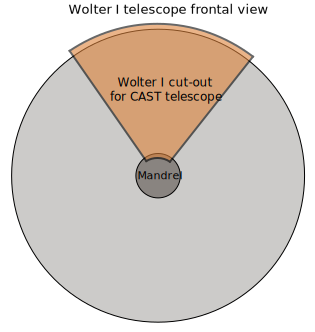
\includegraphics[height=6cm]{figures/cast/wolter1-cutout.eps}
  \caption{}
  \label{fig:wolter1-cutout}
\end{figure}

By using only 1/6 of the Wolter I radial reflective area, a pie-slice (figure \ref{fig:wolter1-cutout}), two stacks of mirrors can be used to reflect X-rays to one side. The stack only needs to be high enough to cover the bore opening, but each mirror should also be wide enough. The NuSTAR glass are made in 60\degr\ segments for the inner radii and 30\degr\ segments for the outer radii.

\subsection{Optic geometry considerations}
The geometry of the optic was calculated using the following equation for a Wolter I optic:

\begin{eqnarray}\label{eq:wolter}
  \tan(4\alpha) = \frac{\rho}{f},
\end{eqnarray}

where $\alpha$ is the angle of reflection of each mirror, $f$, is the focal length and $\rho$ is the radius between center of optic and the midpoint between parabolic and hyperbolic mirror (figure \ref{fig:wolter1-diagram}). The center of the bore will need an off-set with the focal plane of the telescope, given by $d$, which is the radius of the bore, $r_{\text{bore}}$, plus the minimum radius of a NuSTAR optic, $r_{\text{min}}$ (figure \ref{fig:optic_and_bore}). The length of the NuSTAR mirrors is $l = 225$ mm.

\begin{figure}
\centering
\begin{minipage}{.5\textwidth}
  \centering
  \includegraphics[width=\linewidth]{figures/cast/axion_search_cast.pdf}
  \captionof{figure}{Diagram of wolter I from side.R1-R5 designated.}
  \label{fig:wolter1-diagram}
\end{minipage}%
\begin{minipage}{.5\textwidth}
  \centering  \includegraphics[width=\linewidth]{figures/cast/axion_search_cast.pdf}
  \captionof{figure}{Show bore-opening with mandrel from front.}
  \label{fig:optic_and_bore}
\end{minipage}
\end{figure}

The focal length $f$ was set to a fixed value of 1.5 m. Using $r_{\text{min}}$ as the first layer radius, $\mathit{R3}_1$, the angle of the first layer, $\alpha_1$, can be calculated using eq. \ref{eq:wolter}. From $\alpha_1$ and $\mathit{R3}_1$, we can calculate $\mathit{R1}_1$, $\mathit{R2}_1$, $\mathit{R4}_1$ and $\mathit{R5}_1$:

\begin{eqnarray}
  \mathit{R2}_1 &=& \mathit{R3}_1 + 0.5 \cdot x_{\text{sep}}\cdot\tan(\alpha),\\
  \mathit{R4}_1 &=& \mathit{R3}_1 - 0.5 \cdot x_{\text{sep}}\cdot\tan(3\alpha),\\
  \mathit{R1}_1 &=& \mathit{R2}_1 + l\cdot\sin(\alpha),\\
  \mathit{R5}_1 &=& \mathit{R4}_1 - l\cdot\sin(3\alpha),
\end{eqnarray}

where $x_{\text{sep}}$ is the distance between the parabolic and hyperbolic mirror. The next layer can be added by setting

\begin{eqnarray}
  \mathit{R3}_2 &=& \mathit{R1}_1 + d_{\text{glass}},
\end{eqnarray}

where $d_{\text{glass}}$ is the thickness of the glass. Thereby the opening will be exactly large enough for all incoming photons to hit the parabolic mirror.


!! setting the focal length to 1.5 m !!


\subsection{Optimising reflective coatings}


\section{Producing coated substrates}


\subsection{Collecting substrates for coating}

\subsection{Coating of substrates}



\section{Assembling coated substrates}


\subsection{Acquiring parts for assembly vacuum vessel}


\section{Installation of optic at CAST}


\subsection{Optic alignment}

\subsection{Tests with 8 keV X-ray source}

\section{Conclusion}
%\section{First light}

%!TEX root = /Users/andcj/Dropbox/Documents/PhD/Thesis/phdthesis.tex
\chapter{Telescope design for the International AXion Observatory (IAXO)}\label{chap:iaxo}

CAST is a third generation axion helioscope and was the first experiment to surpass the astrophysical limit on the axion-photon coupling of \gay\ $\lesssim 10^{10}$ Gev$^{-1}$ in a broad axion mass range. The CAST helioscope search has reached slightly into the part of parameter space predicted by models to be most likely to detect the axion.

To improve on the CAST achievements and reach further into the "axion band" of the parameter space, a more sensitive instrument is required.

\section{IAXO concept}
Considering that the probability of converting a solar axion into a photon in a magnet with magnetic field $B$ and length $L$ is given by\cite{Andriamonje:2007jc,Zioutas:2005jl,Sikivie:1983wx}:

\begin{eqnarray}
  P_{\text{a}\gamma} &=& 2.6\cdot10^{-17}\bigg(\frac{B}{10\text{ T}}\bigg)^2\bigg(\frac{L}{10\text{ m}}\bigg)^2(g_{\text{a}\gamma}\cdot10^{10}\text{\ GeV})^2\mathcal{F},
\end{eqnarray}

where $\mathcal{F}$ is the coherence length:

\begin{eqnarray}
  \mathcal{F} &=& \frac{2(1-\cos{qL})}{(qL)^2}
\end{eqnarray}

and $q$ is the momentum transfer. It becomes apparent that in order to improve on the probability of axion-photon conversion, either $B$ or $L$ has to be improved. In CAST $B \leq 9$ T, and it is already the limit of what is achievable with a large superconducting magnet. The magnet could be made longer, but it also has to be able to point at the sun and the improvement will only be a factor of two. The last possibility is to increase the collecting area of the magnet, so instead of two bores of 43 mm diameter like in CAST, bore diameter could be prioritized over magnetic field. An optimal design for a new magnet was identified\cite{Irastorza:1340820} in the ATLAS magnet for LHC\cite{Collaboration:1997vu}, since it achieves a much larger cross section area by having much larger bores.

Using the toroidal design of the ATLAS magnet, a proposed design gave a magnet 25 m long with a peak magnetic field of $B \leq 5.4$ T, by the use of eight one meter wide and 21 m long racetrack coils. The magnet bores would be each 600 mm diameter and could be placed either inside the coils or between them. A higher magnetic field could be achieved by placing the bores inside the coils, but the coils would themselves block converted X-ray photons from reaching the detector, see figure \ref{fig:toroid_field}. Eight magnet bores of 25 m length, 600 mm diameter and $B \leq 5.4$ T, would equal approximately the same $BL$ as CAST, but achieving a cross section area of $\sim2.3$ m$^2$ compared to $3\cdot10^{-3}$ m$^2$ for CAST.

\begin{figure}[!h]
  \center
\includegraphics[width=0.8\linewidth]{figures/iaxo/toroid_field.pdf}
\caption{\footnotesize Illustration of the bore configurations with respect to superconducting coils in the IAXO magnet. Having the bores inside the coils (a) will give a stronger magnetic field, but X-ray telescopes at the end of each bore will be blocked in the center by the coil. With the bores between the coils (b), the magnetic field is not as strong, but the entire bore cross section area is usable. From \cite{Irastorza:2013uu}.}\label{fig:toroid_field}
\end{figure}

The large cross section will require X-ray telescopes to focus converted X-ray photons into detectors, as low-background detectors with such a large collecting area would not be possible. A design of the IAXO helioscope\cite{Vogel:2013we,Shilon:1501687,Irastorza:2012tt} with X-ray telescopes at each magnet bore can be seen in figure \ref{fig:iaxo_helioscope}. The proposed design of IAXO can achieve much higher inclination than CAST ($\pm$25\degr\ vs. $\pm$8\degr), so will be able to folow the sun for longer periods ever day.

\begin{figure}[!h]
  \center
\includegraphics[width=0.8\linewidth]{figures/iaxo/iaxo_helioscope.pdf}
\caption{\footnotesize Schematic view of the IAXO helioscope. The cryostat containing the toroidal superconducting magnet is placed on a turret with complete 360\degr\ of rotation. Eight telescopes with separate detectors are placed at the end. Flexible lines feeds the magnet with liquid He and power. A fixed dome can cover the whole experiment as axions will not interact with the walls. From \cite{Armengaud:2014eo}.}\label{fig:iaxo_helioscope}
\end{figure}

IAXO will be able to achieve a sensitivity five orders of magnitude compared to CAST, which translates into \gay values as low as \gay\ $\sim5\cdot10^{-12}$ GeV$^{-1}$ for axion masses up to $\sim$0.01 eV, as can be seen in figure \ref{fig:iaxo_search}. The experiment would explore deep into the ALP\footnote{Axion-like particle} and axion parameter space, and even without detection would exclude a large region of QCD axion phase space that is completely unexplored. A detection of any fundamental pseudo-scalar particle would be groundbreaking for particle physics.

\begin{figure}[!h]
  \center
\includegraphics[height=8.5cm]{figures/iaxo/iaxo_axion_search.pdf}
\caption{\footnotesize The expected sensitivity of IAXO with currently excluded refions by CAST and ADMX\cite{Asztalos:2001ty} shown. Refer to fig. \ref{fig:axion_search_cast} for labels of the various regions. From \cite{Irastorza:2013uu}.}\label{fig:iaxo_search}
\end{figure}

\section{X-ray telescope design}
In appendices \ref{pap:axion_spie} and \ref{pap:iaxo_concept}, the design of X-ray telescopes for IAXO is described in detail. Using a modified version of the software developed for the CAST optic, a geometry for a NuSTAR-like optic was found.

The IAXO helioscope will be without the limitations in telescope focal length found in the CAST experiment. The design of
 the telescope should however take into consideration the focal spot size resulting from the optic figure error and angular size of the sun. A longer focal length will increase the throughput of the optic, but will also increase the spot size. An algorithm for optimising the focal length was developed, and a 5 m focal length was found to be the optimal solution.

An additional outcome of the shorter focal length is the easier production demands as a result of fewer glass substrate layers in the optic. A 10 m focal length would require 235 glass substrate layers, compared to 133 layers for NuSTAR which has a similar focal length but only 400 mm diameter. With eight telescopes, that would result in $\sim8,000\cdot8=64,000$ glass substrates for IAXO, which is a large undertaking considering that the coating of $\sim6,000$ glass substrates for NuSTAR took a year full time at the DTU Space coating facility. The 5 m focal length would only require 110 glass substrate layers; it would also put less demand on the structure of vacuum tubes going from telescopes to detectors (see figure \ref{fig:iaxo_helioscope}).

\section{Coatings for IAXO X-ray telescopes}
Eight telescopes with 110 glass substrate layers is still a large undertaking for the coating chamber at DTU Space. The coating of all glass substrates would not be achievable in the 2.5 year time span set by the Letter of Intent\cite{Irastorza:2013uu} submitted to CERN in 2013. New coating chamber(s) would be needed and a year is set aside for the setup of new coating facilities before production begins.

For a large-scale coating production on curved glass substrates, a departure from the design of the coating facility at DTU Space is required. One of the main drawbacks is the inability to change samples for coating without opening the chamber completely. After closing the chamber with new samples inside, five to six hours of pumping is required in order to achieve the base pressure of $\leq 2\cdot10^{-6}$ Torr. A NuSTAR like coating that takes 12 hours to coat, requires 18 hours after samples are put into the chamber. A load lock system would be able almost remove the pump-down time.

The coatings for IAXO are similar CAST and ATHENA coatings, 5--15 bilayers layers of 5--20 nm d-spacing, so each coating is relatively quick. The coating chamber at DTU Space has a rotational geometry, an advantage when coating many ($>100$) bilayers, but that is not required for IAXO. Instead it is advantageous to make a linear coating system, where substrates a placed on $\sim$60x60 cm$^2$ horizontal sample holder plates and the plates can be stacked in a hopper-like system. A hopper with 10 plates each holding 6--8 samples could be placed in a load-lock and the system would automatically take out the plates to be coated one at a time. The plates would move horizontally past a number of cathodes, where one layer would be deposited on the way out and one layer on the way back, resulting in one bilayer per return trip. Each plate can be applied a different coating based on the velocity of the plate across the cathode plasma and the cathode power setting. The number of bilayers is set by the number of return trips of a plate.

The cathodes should be linear magnetrons of $\sim$80 cm length, placed horizontally and pointing down. Increased uniformity of coating on the cylindrically curved substrates that would be used for IAXO can be achieved by measuring the curvature of each sample in the chamber immediately before coating using a distance sensor. The cathodes could then automatically increase/decrease power as the samples move by according to the curvature of each sample.

Using two chambers of the design proposed above, the $\sim$30,000 substrates can be coated within the two year time span set by the Letter of Intent.

\section{Conclusion}
In this chapter was described shortly the considerations taken in the design of X-ray telescopes for IAXO. Using a modified version of the software used to design the CAST XRT, telescopes suitable for IAXO were designed and an optimal focal length of 5 m were found.

IAXO is an international collaboration involving 29 institutes from across the world, each playing a part in the design, construction and operation of the experiment. The main barrier at the time of writing is the funding of the $\sim$100M \euro experiment, but both European and American institutions and agencies have expressed their interest in the project.

The Letter of Intent for IAXO submitted in 2013, was approved by CERN in spring of 2014 and IAXO then became an official experiment at CERN. The IAXO collaboration was encouraged by CERN to take the next steps toward a technical design report that would include R\&D on magnet, detectors and X-ray telescopes.

%!TEX root = /Users/andcj/Dropbox/Documents/PhD/Thesis/phdthesis.tex
\chapter{!!!!!!Conclusion and outlook}
hjgirejg reio

\appendix

%%%%%%%APPENDIX CHAPTERS INCLUDE%%%%%%%%%%%%%%%%%%%%%%%%%%%%%%%%%%%%%%%%%%%%%%

% Appendix A, B, ...

\renewcommand{\papertitle}{Preliminary coating design and coating developments for Athena}
\chapter{\papertitle}
\label{pap:PREL_Athena}
\markboth{\appendixname\ \thechapter}{\papertitle}
\emph{Preprint}
%Publication printed in {\em Proc.\ SPIE,\ Optics for EUV, X-Ray, Gamma-Ray Astronomy V}.

\includepdf[pages=-,scale=.9,pagecommand={}]{papers/prel_athena.pdf}
\newpage\mbox{} % Blank side s� artiklen starter p� et ulige sidetal
\markboth{}{}

\renewcommand{\papertitle}{Development and characterization of coatings on silicon pore optics substrates for the Athena Mission}
\chapter{\papertitle}
\label{pap:Athena_2012}
\markboth{\appendixname\ \thechapter}{\papertitle}
\emph{Preprint}
%Publication printed in {\em Proc.\ SPIE,\ Space Telescopes and Instrumentation 2012: Ultraviolet to Gamma Ray}.

For this paper I produced the coated substrates as well as performed XRR measurements at DTU Space and the BESSY II synchrotron in Berlin.

\includepdf[pages=-,scale=.9,pagecommand={}]{papers/spo_2012_desiree.pdf}
\newpage\mbox{} % Blank side s� artiklen starter p� et ulige sidetal
\markboth{}{}


\renewcommand{\papertitle}{X-ray optics for axion helioscopes}
\chapter{\papertitle}
\label{pap:axion_spie}
\markboth{\appendixname\ \thechapter}{\papertitle}
\emph{Preprint}
%Publication printed in {\em Proc.\ SPIE,\ Optics for EUV, X-Ray, Gamma-Ray Astronomy VI}.

\includepdf[pages=-,scale=.9,pagecommand={}]{papers/axion_spie.pdf}
\newpage\mbox{} % Blank side s� artiklen starter p� et ulige sidetal
\markboth{}{}


\renewcommand{\papertitle}{Conceptual design of the International Axion Observatory (IAXO)}
\chapter{\papertitle}
\label{pap:iaxo_concept}
\markboth{\appendixname\ \thechapter}{\papertitle}
Publication printed in {\em Journal\ of\ Instrumentation}. It is a retooled version of the Letter of Intent that was submitted to the CERN SPSC in summer 2013.\\
\\
Presented in this thesis is a shorter version of the paper, only representing the work that I did. The full paper is 46 pages and a large part is outside the field of X-ray optics. First half page is part of an earlier section and cut out here.

\includepdf[pages=22-27,scale=.9,pagecommand={}]{papers/iaxo_annotated.pdf}
\newpage\mbox{} % Blank side s� artiklen starter p� et ulige sidetal
\markboth{}{}

\chapter{X-ray principles}\label{chap:xray_appendix}
% \renewcommand{\papertitle}{X-ray principles}
% \markboth{}{}
% This chapter is taken from my own master thesis from 2010 and describes the principles of X-ray reflection from imperfect surfaces and interfaces.
%
% Anders C. Jakobsen, Developing Supermirror Optics for Hard X-rays, \emph{Master thesis}, University of Copenhagen, 2010.
%
% \newpage\mbox{} % Blank side s� artiklen starter p� et ulige sidetal
% \markboth{\papertitle}{}

% \section{X-ray principles}
The development of multilayer mirrors for X-ray focusing requires the ability to measure the properties of the deposited films. A number of techniques can be used, but by far the most practical is X-Ray Reflectometry (XRR) that allows for relatively fast ($\sim$ 20 mins. in our setup) non-destructive measurements and gives information about thicknesses, densities and interlayer imperfections.

\section{Reflection from a surface}
An X-ray photon propagating through one medium and hitting the surface of another medium will interact with the surface by changing direction, either as reflection or refraction. The principle of refraction is explained by \emph{Snell's Law}
\begin{eqnarray}
	n_1 \cos{\theta_1} = n_2 \cos{\theta_2}
\end{eqnarray}

where $n_1$ and $n_2$ are the refractive indexes of the first and second medium respectively. $\theta_1$ and $\theta_2$ are the grazing angle of the incident photon and grazing angle of refracted photon respectively.\\

For an incident plane harmonic wave propagating in the direction $\mathbf{K}$, the electric field can be described as
\begin{eqnarray}
	\mathbf{E} = E_0 \mathrm{e}^{i(\mathbf{K}\cdot \mathbf{r}-\omega t)}
\end{eqnarray}

with amplitude $E_0$. The magnetic field in the plane harmonic wave, $\mathbf{B}$, is perpendicular to the electric field.\\

There are two polarization modes when considering a plane harmonic wave incident on a surface, either the polarization is Transverse Electric (TE) or Transverse Magnetic (TM). In the TE mode, the electric field is perpendicular to the plane of incidence, and in the TM mode the magnetic field is perpendicular to the plane of incidence. Any combination of polarization of the two modes can be considered a superposition of the two, so it is enough to look at only the TE and TM modes. And since for small angle grazing incidence X-ray cases the two are nearly identical\cite{pedrotti:1993}, only the TE mode will be considered from here on. \\

As the incident wave hits the surface it can either reflect or refract and the electric field of the reflected, $E_r$, and refracted, $E_t$, waves are
\begin{eqnarray}
	\mathbf{E_r} & =  & E_r \mathrm{e}^{i(\mathbf{K}\cdot \mathbf{r}-\omega t)},\\
	\mathbf{E_t} & =  & E_t \mathrm{e}^{i(\mathbf{K}\cdot \mathbf{r}-\omega t)}.
\end{eqnarray}

The relation between reflection, refraction and incident wave is described by the reflectivity amplitude, $r$, and transmittivity amplitude, $t$. They are calculated from the electric field amplitudes and their projection parallel to the surface
\begin{eqnarray}
	E \sin{\theta} - E_r \sin{\theta} &=& n E_t \sin{\theta_t}.
\end{eqnarray}

and provide the Fresnel equations
\begin{eqnarray}\label{fresneleq}
	r & \equiv & \frac{E_r}{E} = \frac{\sin{\theta}-n \sin{\theta_t}}{\sin{\theta}+n \sin{\theta_t}}, \\
	t & \equiv & \frac{E_t}{E} = \frac{2\sin{\theta}}{\sin{\theta}+n \sin{\theta_t}}
\end{eqnarray}

that describes the reflectivity and transmittivity from an interface between a medium with refractive index of unity (vacuum/air) and another medium with refractive index $n$.

\section{Reflection from a thin film}
Further evolving the Fresnel equation to describe $r$ and $t$ from an interface between two mediums with refractive indexes $n_i$ and $n_j$ yields
\begin{eqnarray}
	r_{ij} & \equiv & \frac{E_i^{'}}{E_i} = \frac{n_i\sin{\theta_i}-n_j \sin{\theta_j}}{n_i\sin{\theta_i}+n_j \sin{\theta_j}}, \label{reflectivitetinterface}\\
	t_{ij} & \equiv & \frac{E_t}{E_i} = \frac{2 n_i\sin{\theta_i}}{n_i\sin{\theta_i}+n_j \sin{\theta_j}}.\label{transmittivity}
\end{eqnarray}

Here $E_i$ is the electric field amplitude incident on the interface in medium $i$ and $E_i^{'}$ is the reflected electric field amplitude in medium $i$. $E_j$ is the refracted electric field amplitude in medium $j$.\\

For a thin film on a substrate, there are three mediums: First air ($n_0$), then film ($n_1$) and finally substrate ($n_s$). An incident X-ray photon acting on a thin film have an infinite number of ways to interact with the interfaces. Either the photon is reflected from the first layer, so $r_{01} = 1$, or it is transmitted through the first layer and reflected from the next, or transmitted, then reflected, then reflected and so on. All those possibilities are described by a geometric series
\begin{eqnarray}
	r_{\mathrm{thin film}} = r_{01} + t_{01}t_{10}r_{1s}\mathrm{e}^{2 i \beta_i}\sum_{m=0}^{\infty}(r_{10}r_{12}\mathrm{e}^{2 i \beta_i})^m
\end{eqnarray}

where $\mathrm{e}^{2i\beta_i}$ is a phase factor to correct the phase of the waves before being added up and $\beta = 2 \pi d_i n_i \sin{\theta_i}\lambda^{-1}$. Noting that $\sum_{m=0}^{N}k^n = \frac{1 - k^n}{1-k}$ becomes $\sum_{m=0}^{\infty}k^n = \frac{1}{1-k}$ for $|k| < 1$, the series can be simplified to
\begin{eqnarray}
	r_{\mathrm{thin film}} = r_{01} + t_{01}t_{10}r_{1s}\mathrm{e}^{2i\beta_i}\frac{1}{1-r_{10}r_{12}\mathrm{e}^{2i\beta_i}}
\end{eqnarray}

and finally give
\begin{eqnarray}
	r_{\mathrm{thin film}} = \frac{r_{01} + r_{12}\mathrm{e}^{2i\beta_i}}{1-r_{10}r_{12}\mathrm{e}^{2i\beta_i}} \label{slabapprox}
\end{eqnarray}

\section{Reflection from multilayers}
For calculating the reflectivity from a multilayer stack a method such as the Kinematical approximation can be used. But the approximation have the downside of only being able to calculate for multilayers where the bilayer thickness (d-spacing) is constant throughout the multilayer stack. \\
Since the development of X-ray optics involves making multilayers where the d-spacing change through the stack, it is more appropriate to compute an iterative model using the formula just derived in Eq. (\ref{slabapprox}) . The software used in modeling specular reflectivity from a multilayer is IMD\cite{Windt:1998tb}. It takes the two formulas
\begin{eqnarray}\label{fresnelcoef}
	r_i &=& \frac{r_{ij}+r_j\mathrm{e}^{2 i \beta_i}}{1+r_{ij}r_j\mathrm{e}^{2 i \beta_i}},\\
	t_i &=& \frac{t_{ij}t_j\mathrm{e}^{2 i \beta_i}}{1+r_{ij}r_j\mathrm{e}^{2 i \beta_i}}\\
\end{eqnarray}

to calculate the $i$'th layer where $r_{ij}$ is Eq. (\ref{reflectivitetinterface}) and $t_{ij}$ is Eq. (\ref{transmittivity}). Since the $j$'th layer is the layer below $i$, the software calculation can start from the bottom layer, the substrate, where there is no reflectivity from below. From the bottom layer, the software works it way up recursively through each layer, adding up the reflectivity and transmittivity. That is the Paratt recursive method\cite{Parratt:1954wb}.\\
The energy reflected from or transmitted through the film is denoted as the reflectance $R$ and transmittance $T$
\begin{eqnarray}
	R &=& |r|^2,\\
	T &=& \mathrm{Re}\Bigg\{\frac{n_s \sin{\theta_s}}{n_a \sin{\theta_a}}\Bigg\}|t|^2.
\end{eqnarray}

The IMD software approximates the absorptance, $A$, using $R$ and $T$
\begin{eqnarray}
	A = 1-R-T
\end{eqnarray}

where A is the energy absorbed by the entire film.

\section{Reflectivity changes due to imperfections in the interface}
In experimental cases, the interface between two mediums, or materials, is not completely smooth. The imperfections can be distinguished into two types. Either by atoms in the structure that have been deposited unevenly to create 'hills' and 'valleys' in the surface, which is called pure roughness, $\sigma_p$. The other type is diffuse roughness, $\sigma_d$, caused by diffusion of atoms from one material into another.\\
To describe the roughness, the interface can be seen as not an abrupt change of refractive index, but as a profile function, $p(z)$\cite{Stearns:1989va}, that takes the normalized average value of the dielectric function, $\varepsilon(\mathbf{x})$, in the $z$ direction, where
\begin{eqnarray}
	p(z) = \frac{\int \int \varepsilon(\mathbf{x})dxdy}{(\varepsilon_i-\varepsilon_j)\int \int dxdy}, \\
	\varepsilon(\mathbf{x}) = \Bigg\{
	\begin{array}{rl}
		\varepsilon_i, & z \rightarrow + \infty \\
		\varepsilon_j, & z \rightarrow - \infty \\
	\end{array}.
\end{eqnarray}

Taking the Fourier transform of $dp/dz=w(z)$ gives $\tilde{w}(s)$, where $s = 4 \pi \sin{\theta}/\lambda$. As Stearn found out, multiplying the Fresnel coeffiecients from Eq. (\ref{fresnelcoef}) with $\tilde{w}(s)$ gives the approximate reflectance including loss from imperfect interfaces. That gives the modified Fresnel coefficients used by IMD:
\begin{eqnarray}
	r_{ij}^{'} = r_{ij} \tilde{w}(s).
\end{eqnarray}

The most commonly used interface profile, $p(z)$, is the error function
\begin{eqnarray}
	p(z) = \frac{1}{\sqrt{\pi}}\int_{-\infty}^z \mathrm{e}^{-t^2/(2\sigma_{rms}^{2})}dt
\end{eqnarray}

which after taking the Fourier transform of $dp/dz$ becomes
\begin{eqnarray}\label{interfacefunction}
	\tilde{w}(s) = \mathrm{e}^{-s^2\sigma_{rms}^2/2}.
\end{eqnarray}\\

The width of the interface function is denoted by $\sigma_{rms}$ that is the root mean square of $\sigma_p$ and $\sigma_d$, so
\begin{eqnarray}
	\sigma_{rms} = \sqrt{\frac{\sigma_p^2 + \sigma_d^2}{2}}.
\end{eqnarray}

% \section{Diffuse reflection}\label{diffuserefl}
% In the previous section only specular reflection was covered and dealt with by reducing the problem to a one-dimensional one without worrying about scattering. In case of roughness, there was merely an approximate factor to account for loss of reflection.\\
% Roughness in an interface will cause scattering outside the specular reflection, which can be modeled either using the Born Approximation (BA) or Distorted Wave Born Approximation (DWBA)\cite{Sinha:1988uu}. The regular BA is suitable for looking at scattering away from the critical angle, where scattering is considered a weak interaction and multiple refraction effects are negligible. When looking at multilayers, the BA is not suitable since it does not take multiple reflections into account.\\
% The DWBA is more suitable for multilayers, where total external and internal reflections near the critical angle are taken care of. Every imperfect interface is regarded as a perturbation. Sinha et al.\cite{Sinha:1988uu} worked out the DWBA for singlelayer and later the model was expanded to include multilayer systems\cite{Stearns:1998wn,Kopecky:1995uy,Holy:1993p5469}. In this section the formulas will not be derived, but the final formula presented and explained.\\
%
% The measured intensity in a scattering experiment is explained by
% \begin{eqnarray}
% 	I = I_0 \int_{\Omega_{detector}} \frac{d\sigma}{d\Omega} d\Omega.
% \end{eqnarray}
%
% where $I$ is the measured intensity, $I_0$ the incident intensity and $\frac{d\sigma}{d\Omega}$, the differential cross section. For non-specular reflectivity, the incoherent differential cross section is used, as derived for multilayers by Holy et al.\cite{Holy:1993p5469}
%
% \begin{eqnarray}\label{holyeq}
% 	\Bigg(\frac{d\sigma}{d\Omega}\Bigg)_I &=&\frac{Sk^4}{16\pi^2}\sum_{i=1}^N |n_{i}^2 - n_{i+1}^2|^2  \nonumber \\
% 	 &\times&|(t_{1,i+1}t_{2,i+1}+r_{1,i+1}r_{2,i+1})\mathrm{e}^{\frac{-(\sigma_i q_{0z,i+1})^2}{2}} \nonumber  \\
% 	 &+&(t_{1,i+1}r_{2,i+1}+t_{2,i+1}r_{1,i+1})\mathrm{e}^{\frac{-(\sigma_i q_{1z,i+1})^2}{2}}|^2 \\
%   &\times& C_i^{'} (q_x,q_y)
% \end{eqnarray}
%
% which is the simplified version applicable when $|q_{z,i+1}\sigma_2|^2 << 1$. The first factor contains the area $S$ hit by the incident beam and the wave number $k = 2\pi/\lambda$. Next is the sum that iterates over all $N$ layers from bottom layer up. The factor $|n_{i}^2 - n_{i+1}^2|$ takes the square of the index of the current layer and subtracts the square of the index of the layer above.\\
% Next is the Fresnel equations (Eq. (\ref{fresneleq})) which are multiplied by a modified interface function similar to Eq. (\ref{interfacefunction}) except the use of $q_{0z,i+1}$ and $q_{1z,i+1}$.\\
% The two wave vector transfers correspond to two different processes that occurs during diffuse scattering. The term $t_{1,i+1}t_{2,i+1}$ express the scattering from the transmitted wave with amplitude $t_{1,i+1}$ into the wave with amplitude $t_{2,i+1}$. The wave vector change corresponding to that interaction is $\mathbf{q}_{0,i+1} = \mathbf{K}_{2,i+1}-\mathbf{K}_{1,i+1}$. Refer to figure \ref{fig:holykvector}.\\
% And for $t_{1,i+1}r_{2,i+1}$, it is the scattering from the transmitted wave with amplitude $t_{1,i+1}$ into the reflected wave with amplitude $r_{2,i+1}$ and the wave vector transfer for that is $\mathbf{q}_{1,i+1} = \mathbf{K}_{2,i+1}^{'}-\mathbf{K}_{1,i+1}$.
%
% \begin{figure}[!ht] % holykvector
% 	\centering
% 		\includegraphics[height=2.2in]{figures/xray_app/holykvector.pdf}
% 	\caption{Cross section of $N$-layer multilayer on substrate with visualization of wave vectors on the surface and in the $j$'th layer. From \cite{Holy:1993p5469}.}
% 	\label{fig:holykvector}
% \end{figure}
%
% The last part in Eq. (\ref{holyeq}), $C_i^{'} (q_x,q_y)$, is the two dimensional Fourier transform of the correlation function, $C_i$
% \begin{eqnarray}
% 	C_i^{'} (q_x,q_y) &=& \int_S dxdy C_i(x,y)\mathrm{e}^{-i(xq_x +yq_y)}.
% \end{eqnarray}
%
% The correlation function is often described with a statistical distribution of a self-affine fractal-like surface\cite{Sinha:1988uu}
% \begin{eqnarray}
% 	C_i (x,y) = \sigma^2 \mathrm{e}^{-(\rho/\xi)^2h}
% \end{eqnarray}
%
% where $\sigma$ is the rms roughness of the surface and $\xi$ is a lateral correlation length which is an expression for how large an area is needed to measure before $\sigma$ is constant. If the roughness is periodic along the surface, $\xi$ is the length of the period. $h$ is the Hurst parameter that describes the jaggedness of the surface between 0 and 1. For $h=0.5$ the function becomes exponential and for $h=1$ it is Gaussian. So the higher the Hurst parameter, the smoother the surface.\\
%
% The software used for modeling diffuse reflectivity is BEDE\cite{Wormington:1992vm}, which uses Eq. (\ref{holyeq}) for the off-specular part. In this work, measurements of diffuse reflectivity were done by transverse scans, where the sum of the ingoing angle, $\theta_{I_0}$, and outgoing angle, $\theta_I$, is constant ($\theta_{I_0} + \theta_I=\mathrm{constant}$). \\
%
% \begin{figure}[!ht] % double reflected
% 	\centering
% 		\includegraphics[height=2in]{figures/xray_app/transverse.pdf}
% 	\caption{Simulation of a transverse XRR scan calculated in BEDE of a 400 \AA\ W singlelayer on a silicon substrate with roughness of 4 \AA, correlation length of 200 \AA\ and Hurst parameter of 0.7. }
% 	\label{fig:transverse}
% \end{figure}
%
% An example of a simulated transverse reflection can be seen in figure \ref{fig:transverse}. The peaks on both sides of the graph are Yoneda peaks\cite{Yoneda:1963tr} and arise from multiple scattering processes when either $\theta_{I_0}$ or $\theta_I$ equals the critical angle, $\theta_c$.

\chapter{Multilab control software}\label{sec:ml_software}
In the years before moving the DTU Space multilab to DTU campus, it became apparent that a completely new software solution was needed for the coating facility. The software controls all stepper motors (cathode shutters and sample ring), gas flow controllers,  cathode power supplies as well as pressure gauge communication.

The original software was made in Visual Basic 6, which Microsoft stopped supporting in 2008. Features that were not build into the software from the start was bolted on at a later stage, resulting in some files with thousands of lines of uncommented code. VB6 also has the drawback that it is single threaded so only one command can be executed at a time, which means that none of the instruments could be read for the log file if e.g. the sample ring was moving. So checking whether there was a plasma dropout on a cathode was not possible while coating a layer, something that can take 30+ minutes.

Everything in the original software solution was controlled in a graphical user interface which made it easy to use, but would only allow for preprogrammed coating types to be made. When it came to make coating investigations for the Athena mission, the linearly graded coatings with top and bilayer required being in front of the computer during the process. For every layer, it was necessary to manually type in a new sample ring speed and start the movement. The coatings took on average 2-3 hours, so it became clear that a new solution was necessary.

\section{Considerations on the new software solution}
Considering the observations from above, a list of requirements for new software was made:

\begin{description}
  \item[Software should run on Linux] To remote control the coating facility in the old software solution, it was necessary to run a remote desktop to control the graphical user interface. The remote desktop requires a relatively large amount of internet bandwidth, something that is not always available. The new software should be controllable over a remote SSH connection using a Bash shell or similar.
  \item[Software should log continuously] Output from cathode power supplies, pressure gauges and flow meters should be read every 5 seconds during a coating. Between coatings, the pressure gauges should be read every 5 seconds and written to a web server. That allows for checking chamber status on a smart phone or computer connected to the internet.
  \item[A coating run should be described in a script] Instead of predefined coating types, the scripts make it possible to produce completely custom multilayer coatings.
  \item[Software should preferably be open source] Open source software is often well documented and flexible. An open source programming language with plenty of extra packages could be Python.
\end{description}

The first attempts at creating new software was directed at Python, since that is just about the most well-documented programming language on the internet, and also where I have the most experience.

It became clear after a while that the real problem was satisfying the second requirement in the list above. All instruments controlled by computer in the multilab are communicated with using serial connections, which will block a line until a command is received by an instrument and a response is returned. In some instruments the response time is up to a second and for the stepper motors, a response is not returned until movement is complete. That is the reason why the old software was unable to read any outputs during the movement of the sample ring.

Python is a single threaded scripting language, so all commands are executed sequentially. There are however software packages for Python that can spawn subprocesses from a queue and read the output of those into another queue. A specific package for multithreading serial communication is Twisted for Python, but after moderately successful attempts it was clear that the solution would be too difficult. The software should be flexible and making a multithreaded python solution with queue systems was both too much work and a bit like reinventing the wheel.

The choice in the end fell on SPEC, a software package for X-ray diffraction setups. SPEC is not open source, but requires a license. SPEC is widely used in synchrotron beamlines across the world, and also in the X-ray lab at DTU Space. It is an extremely flexible piece of software, specifically designed to talk to a wide range of instruments at X-ray beamlines. Many types of hardware can be controlled directly from SPEC without the need for drivers, since a direct hardware level communication protocol is build into the software. Commands are typed in on a command line, but can also written into text files (scripts) and the commands can then be executed sequentially by SPEC.

\section{Software architecture of new Multilab control program}
SPEC is, like Python, single threaded. There are however build-in procedures for communicating through the serial protocol and a range of other protocols. SPEC also has the ability to run as a server so commands can be issued to the software using sockets on the system level. By running three separate instances of SPEC at the same time, it became possible to constantly communicate with instruments, write to a logfile, and control the chamber from a main program. The software is set up like the following:

\begin{description}
  \item[SPEC (main program)] The main program, where user-level commands can be typed in. Coating macros are executed from this program. The program has direct control with stepper motors using text-based serial communication\footnote{To use SPEC most efficiently, a direct hardware-level communication should be initiated between SPEC and motor controller. However, the motor controller would have to be supported on the hardware-level by SPEC, which is not the case for the current hardware in the Multilab. If a new motor controller is procured, it should be on the list of hardware supported by SPEC. (\emph{http://www.certif.com/hdwdevices.php?family=motor})}.
  \item[ControlServer] The control program. It has direct access to cathode power supplies, gas flow controllers and pressure gauges. SPEC and LogClient will get status and control the instruments through ControlServer by socket commands.
  \item[LogClient] The logging program. It gets data from the ControlServer every five seconds and writes the data to a file. If a coating is starting, it will make a new folder in the \verb'~/logs' directory named by time and date. In that directory it will make a log file (\verb'logfile.txt') for the coating and also a log of the commands typed in by a coating macro (\verb'coatinglog.txt').
\end{description}

These three programs run continuously side-by-side, and will make sure that there are no interruptions in the logging during a coating run. Each command to control any part of the instruments are described in the \verb'site.mac' macro files of each program and auxiliary macro files for e.g. power supplies and pressure gauges. All commands are divided into system-level and user-level commands. System-level commands are called like this:

\begin{verbcode}
  SPEC> output = getpoweroutput(#)
\end{verbcode}

This command will get the output of cathode \verb'#' and put the result in the variable \verb'output'. The system-level commands \emph{can} be used by the user, but \emph{should not}. Instead they are used inside user-level command macros, so a user-level command looks like this:

\begin{verbcode}
  SPEC> getpoweroutput 1
  Current power output of cathode 1: 450 W
\end{verbcode}

This makes it easier to type commands into SPEC, as commands can be autocompleted by using the tabulator key. If a command needs one or several parameters following it and not enough/too many are given, it will respond with an error and a description of the parameters needed.

Log files produced continuously by the LogClient program are fetched by a web server at DTU Space that will make a plot of pressure and cathode power output every 30 seconds. A plot from Sept. 14th 2014 can be seen in figure \ref{fig:chamber_pressure}. The logfile holds up to 50,000 lines of data, which corresponds to $\sim$3 days of data collected every five seconds. In the plot can be seen both the curve corresponding to the cold cathode pressure gauge (red line) and the baratron pressure gauge (green line). The cold cathode works well at both low and high pressure, but some of the functional parts can be coated over during a coating, so a valve closes off to that gauge during coating. The baratron only works between $10^{-1}$ Torr and $2\cdot10^{-4}$ Torr, but is more precise and also works during a coating.

\begin{figure}[htbp]
  \centering
    \includegraphics[width=0.8\linewidth]{figures/chamber/pressure.png}
  \caption{\footnotesize Plot representing the output from the continuous logging of chamber pressure. Red line is the pressure measured by a combined cold-cathode/penning gauge, that works well under both atmospheric pressure and low pressure. It will not function well during a coating. Green line is the MKS Baratron pressure gauge, that is precise in the $2\cdot10^{-4}$ -- $5\cdot10^{-2}$ Torr range.}
  \label{fig:chamber_pressure}
\end{figure}

The web server that continuously fetches the log file from the coating computer also gets information from the X-ray measurement computer in the basement. Information about measurement status and progress is posted to the same web site. This makes it possible to get the status about all the labs by a quick glance to the web site. The script running on the web server also has the option to send out a mail to pre-defined recipients if the pressure in the chamber is low enough to start a coating. This proved handy during the NuSTAR coatings, where coatings had to be started in the middle of the night. The web site and script running on the web server were produced during the NuSTAR coating campaign to make the production process easier.

The cathode shutters and ring are all controlled by the same motor controller, and is communicated to over the same serial cable. That is however opaque to the user. In order to open or close a specific shutter, the command \verb'osh #' or \verb'csh #' should be given for opening and closing shutter \verb'#', respectively. Alternatively, all shutters can be opened or closed using \verb'openallshutters' and \verb'closeallshutters'. The ring can be controlled using the commands \verb'mra speed angle' or \verb'mr speed steps', the first of which moves the ring at the speed given in steps/sec. at an angle given in degrees. The second does the same thing, except for changing the angle for steps. The motor controller has 668,000 steps in a complete rotation of the ring in the chamber and the speed of the ring should be between 0 and 15,000 steps/sec, otherwise the movement precision decreases. In a coating macro, the command \verb'mra speed angle' is used extensively as the main method to move the samples past the cathodes.% In chapter \ref{chap:multilab_details}, an extensive list of commands made for the control software can be found.

\subsection{Interfacing with cathode power supplies}
The power supplies used to run the cathodes in the multilab consist of two Advanced Energy Pinnacle 5/5 DC power supplies and one Advanced Energy Pinnacle Plus+ 5/5 pulsed-DC power supply. Each power supply has two channels, so can run two cathodes at same time. In order to communicate with power supplies, a special protocol running over serial has to be used. All other instruments in the multilab are communicated with by ControlServer and SPEC using basic text commands send over a serial connection.

The protocol is made for connecting all power supplies to the same serial connection, but in the multilab they are connected separately. The protocol requires each command to be packaged in a binary packet that includes power supply hardware address, length of packet, command, data and finally an XOR of the entire packet so the receiver can verify that the whole packet is there. The design of the packet can be seen in figure \ref{fig:ae_packet}. In the header, which is 8 bits long, the first 5 are the address of the power supply (set with a DIP switch on the back) and the remaining 3 bits describe the length of the packet. If the length in the header is set to 7 (111 in binary), the 'optional' byte is used to describe the actual length of the packet. The 'command' byte is a number between 0 and 255 (0 and FFh) in hexadecimal numbers. The 'checksum' byte is an XOR of the entire packet up until the 'chekcksum' byte. When the receiver gets a packet, it will do an XOR of the entire packet including the 'checksum' byte and if the result is 0, the packet is approved and processed.

This packet architecture is used to communicate back and forth between the ControlServer program and the power supplies. If a packet is approved, an ACK is send back in the form of the hex code 06h. The commands for the power supplies can either be to retrieve current status of some parameter, to set a parameter on the power supply, or to execute a command on the power supply. The entire communication protocol is transparent to the user and all user-level control of the power supplies can be achieved by user-level commands only.

\begin{figure}[!h]
  \center
  \includegraphics[width=0.9\linewidth]{figures/chamber/ae_packet.pdf}
\caption{\footnotesize Schematic of the principle of transmission data packets in the Advanced Energy communication protocol. Each number on the white line corresponds to one bit in the data packet, eight bits equals one byte. From \cite{Anonymous:zazNQqcS}}\label{fig:ae_packet}
\end{figure}

\subsection{Coating macro}
To produce a coating in the multilab chamber, a coating macro can be typed up and started in the main SPEC program as soon as the pressure is low enough ($\leq2\cdot10^{-6}$ Torr). An example of a simple coating macro, \verb'coat_singlelayer', can be seen here:

\begin{verbcode}
  def coat_singlelayer '
        if ($# != 1) {
                eprint "Start coating of singlelayer.\n"
                eprint "Usage: coat_singlelayer v(cath3)"
                exit
        }
        coating_start_log
        closevalve
        setflow 1 88
        openflow 1
        openmainflow
        print("Waiting for Ar flow to settle.\n")
        print("(60 seconds).\n")
        sleep(60)
        setpower 3 450
        print("Starting coating.\n")
        mra 90 10000
        sleep(2)
        pson 3
        sleep(5)
        osh 1
        print("Coating material 1, all plates.\n")
        mra -360 $1
        sleep(2)
        csh 1
        sleep(1)
        psoff 3
        mra -90 10000
        sleep(2)
        print("Coating over. Closing flow valve.\n")
        closemainflow
        closeflow 1
        openvalve
        coating_stop_log
        '
\end{verbcode}

Each step in the macro is described here:

\begin{description}
  \item[Error check] The macro starts out with an \verb|if| statement to make sure that there is one parameter after the user has called the macro.
  \item[coating\_start\_log] Sets the variable \verb|coating_starting=1| in the LogClient program and lets it know that it is time to start a log for a new coating.
  \item[closevalve] Closes valve to the cold cathode pressure gauge.
  \item[setflow 1 88] Sets flow output on flow controller 1 to 88 SCCM.
  \item[openflow 1] Opens flow controller 1.
  \item[openmainflow] Opens flow controllers to chamber.
  \item[Text output to user] Feedback should be given to user throughout the coating.
  \item[sleep(60)] Macro will wait for 60 seconds to let the pressure settle at $\sim$2.8 mTorr.
  \item[setpower 3 450] Power output is set to 450 W on power supply output 3, the first output on the second power supply.
  \item[mra 90 10000] Ring is moved 90\degr\ at a speed of 10,000 steps/sec. so the first sample is right before cathode 1.
  \item[pson 3] Power supply 3 is turned on.
  \item[osh 1] Shutter 1 to cathode 1 is opened.
  \item[mra -360 \$1] Ring is moved 360\degr\ at the speed given by the parameter which is set by the user when calling the macro.
  \item[csh 1] Shutter 1 is closed after ring is done moving.
  \item[psoff 3] Power supply 3 is turned off.
  \item[mra -90 10000] Ring is moved back to start position.
  \item[closemainflow] Main flow to flow controllers is turned off.
  \item[closeflow 1] Flow controller 1 flow is turned off.
  \item[openvalve] Valve to cold cathode pressure gauge is opened.
  \item[coating\_stop\_log] Sets the parameter \verb|coating_starting=0| in the LogClient program, which stops logging for that coating.
\end{description}

The macro will coat all samples in the ring with one layer of the material on cathode 1 at the speed given by the parameter after the macro call. Macros in SPEC are given in a C-type language and many types of loops and statements are implemented. The comprehensive manual for SPEC gives a good overview.

If the user wants to make more complicated multilayers, adjusting the macro example above into a graded-d type coating can of course seem daunting. For that reason, subfunctions are implemented that will coat e.g. 90\degr\ of the ring with cathode 3. The principle of the subfunction is as follows:

\begin{enumerate}
  \item From the start position of the ring where sample 1 is placed, the ring will move sample 1 between cathode 2 and 3.
  \item Turn on cathode 3 and open shutter.
  \item Move ring 90\degr\ given by input parameter.
  \item Close shutter 3 and turn off cathode.
  \item Move ring back to start position.
\end{enumerate}

The sample can then be coated by another cathode afterwards. If a larger batch requires coating at the same time, there are similar subfunctions for moving 180\degr\ and 360\degr.

The software also makes it possible to coat four different samples with four different coatings in the same coating run. By placing the samples at four different corners of the ring, each sample can have a coating applied separately. Flexible macros for that purpose are not yet implemented, but a template that can be changed into a specific purpose is the macro
\begin{verbcode}
  SPEC> coat_n_bilayers_4plates
\end{verbcode}
along with subfunction e.g.
\begin{verbcode}
  SPEC> abilayer_4_plates_c2c4($2,$3,$4,$5,$6,$7,$8,$9)
\end{verbcode}
that will coat four different constant-d coatings using cathode 2 and 4. It is possible to change any parameter for the power supplies or flow meters between each sample, so testing out a parameter space becomes significantly faster with this system.

For linearly graded-d coatings, an example is given below that shows the flexibility of the SPEC macro language.

\begin{verbcode}
  for (j=0;j<nlayers;j++){
    printf("\nStarting layer %g.\n",j+1)
    dlayer = dmin+(j)*(dmax-dmin)/(nlayers-1)
    dlayer1 = dlayer*gamma
    dlayer2 = dlayer*(1-gamma)
    speed1 = int(1/((dlayer1-sicorr)/sifact))
    speed2 = int(1/((dlayer2-wcorr)/wfact))
    coat_cath2_180 speed2
    coat_cath4_180 speed1
    }
\end{verbcode}

By defining \verb|nlayers| as the number of layers, \verb|dmin|, \verb|dmax| and \verb|gamma| of the coating along with calibration factors, the macro will for every layer calculate the speed for both materials and coat the correct thickness. Calibration factors are calculated as seen in section \ref{sec:coating_calib} where $a$ for W is \verb|wfact| and $b$ is \verb|wcorr|. The same principle can be used in other types of graded-d coatings, e.g. power-law gradings with $a$, $b$ and $c$ defined in $d_i = a/(b+i)^c$, where $d_i$ is the d-spacing of the i'th layer.

%\chapter{X-ray principles}\label{chap:xray_appendix}
% \renewcommand{\papertitle}{X-ray principles}
% \markboth{}{}
% This chapter is taken from my own master thesis from 2010 and describes the principles of X-ray reflection from imperfect surfaces and interfaces.
%
% Anders C. Jakobsen, Developing Supermirror Optics for Hard X-rays, \emph{Master thesis}, University of Copenhagen, 2010.
%
% \newpage\mbox{} % Blank side s� artiklen starter p� et ulige sidetal
% \markboth{\papertitle}{}

% \section{X-ray principles}
The development of multilayer mirrors for X-ray focusing requires the ability to measure the properties of the deposited films. A number of techniques can be used, but by far the most practical is X-Ray Reflectometry (XRR) that allows for relatively fast ($\sim$ 20 mins. in our setup) non-destructive measurements and gives information about thicknesses, densities and interlayer imperfections.

\section{Reflection from a surface}
An X-ray photon propagating through one medium and hitting the surface of another medium will interact with the surface by changing direction, either as reflection or refraction. The principle of refraction is explained by \emph{Snell's Law}
\begin{eqnarray}
	n_1 \cos{\theta_1} = n_2 \cos{\theta_2}
\end{eqnarray}

where $n_1$ and $n_2$ are the refractive indexes of the first and second medium respectively. $\theta_1$ and $\theta_2$ are the grazing angle of the incident photon and grazing angle of refracted photon respectively.\\

For an incident plane harmonic wave propagating in the direction $\mathbf{K}$, the electric field can be described as
\begin{eqnarray}
	\mathbf{E} = E_0 \mathrm{e}^{i(\mathbf{K}\cdot \mathbf{r}-\omega t)}
\end{eqnarray}

with amplitude $E_0$. The magnetic field in the plane harmonic wave, $\mathbf{B}$, is perpendicular to the electric field.\\

There are two polarization modes when considering a plane harmonic wave incident on a surface, either the polarization is Transverse Electric (TE) or Transverse Magnetic (TM). In the TE mode, the electric field is perpendicular to the plane of incidence, and in the TM mode the magnetic field is perpendicular to the plane of incidence. Any combination of polarization of the two modes can be considered a superposition of the two, so it is enough to look at only the TE and TM modes. And since for small angle grazing incidence X-ray cases the two are nearly identical\cite{pedrotti:1993}, only the TE mode will be considered from here on. \\

As the incident wave hits the surface it can either reflect or refract and the electric field of the reflected, $E_r$, and refracted, $E_t$, waves are
\begin{eqnarray}
	\mathbf{E_r} & =  & E_r \mathrm{e}^{i(\mathbf{K}\cdot \mathbf{r}-\omega t)},\\
	\mathbf{E_t} & =  & E_t \mathrm{e}^{i(\mathbf{K}\cdot \mathbf{r}-\omega t)}.
\end{eqnarray}

The relation between reflection, refraction and incident wave is described by the reflectivity amplitude, $r$, and transmittivity amplitude, $t$. They are calculated from the electric field amplitudes and their projection parallel to the surface
\begin{eqnarray}
	E \sin{\theta} - E_r \sin{\theta} &=& n E_t \sin{\theta_t}.
\end{eqnarray}

and provide the Fresnel equations
\begin{eqnarray}\label{fresneleq}
	r & \equiv & \frac{E_r}{E} = \frac{\sin{\theta}-n \sin{\theta_t}}{\sin{\theta}+n \sin{\theta_t}}, \\
	t & \equiv & \frac{E_t}{E} = \frac{2\sin{\theta}}{\sin{\theta}+n \sin{\theta_t}}
\end{eqnarray}

that describes the reflectivity and transmittivity from an interface between a medium with refractive index of unity (vacuum/air) and another medium with refractive index $n$.

\section{Reflection from a thin film}
Further evolving the Fresnel equation to describe $r$ and $t$ from an interface between two mediums with refractive indexes $n_i$ and $n_j$ yields
\begin{eqnarray}
	r_{ij} & \equiv & \frac{E_i^{'}}{E_i} = \frac{n_i\sin{\theta_i}-n_j \sin{\theta_j}}{n_i\sin{\theta_i}+n_j \sin{\theta_j}}, \label{reflectivitetinterface}\\
	t_{ij} & \equiv & \frac{E_t}{E_i} = \frac{2 n_i\sin{\theta_i}}{n_i\sin{\theta_i}+n_j \sin{\theta_j}}.\label{transmittivity}
\end{eqnarray}

Here $E_i$ is the electric field amplitude incident on the interface in medium $i$ and $E_i^{'}$ is the reflected electric field amplitude in medium $i$. $E_j$ is the refracted electric field amplitude in medium $j$.\\

For a thin film on a substrate, there are three mediums: First air ($n_0$), then film ($n_1$) and finally substrate ($n_s$). An incident X-ray photon acting on a thin film have an infinite number of ways to interact with the interfaces. Either the photon is reflected from the first layer, so $r_{01} = 1$, or it is transmitted through the first layer and reflected from the next, or transmitted, then reflected, then reflected and so on. All those possibilities are described by a geometric series
\begin{eqnarray}
	r_{\mathrm{thin film}} = r_{01} + t_{01}t_{10}r_{1s}\mathrm{e}^{2 i \beta_i}\sum_{m=0}^{\infty}(r_{10}r_{12}\mathrm{e}^{2 i \beta_i})^m
\end{eqnarray}

where $\mathrm{e}^{2i\beta_i}$ is a phase factor to correct the phase of the waves before being added up and $\beta = 2 \pi d_i n_i \sin{\theta_i}\lambda^{-1}$. Noting that $\sum_{m=0}^{N}k^n = \frac{1 - k^n}{1-k}$ becomes $\sum_{m=0}^{\infty}k^n = \frac{1}{1-k}$ for $|k| < 1$, the series can be simplified to
\begin{eqnarray}
	r_{\mathrm{thin film}} = r_{01} + t_{01}t_{10}r_{1s}\mathrm{e}^{2i\beta_i}\frac{1}{1-r_{10}r_{12}\mathrm{e}^{2i\beta_i}}
\end{eqnarray}

and finally give
\begin{eqnarray}
	r_{\mathrm{thin film}} = \frac{r_{01} + r_{12}\mathrm{e}^{2i\beta_i}}{1-r_{10}r_{12}\mathrm{e}^{2i\beta_i}} \label{slabapprox}
\end{eqnarray}

\section{Reflection from multilayers}
For calculating the reflectivity from a multilayer stack a method such as the Kinematical approximation can be used. But the approximation have the downside of only being able to calculate for multilayers where the bilayer thickness (d-spacing) is constant throughout the multilayer stack. \\
Since the development of X-ray optics involves making multilayers where the d-spacing change through the stack, it is more appropriate to compute an iterative model using the formula just derived in Eq. (\ref{slabapprox}) . The software used in modeling specular reflectivity from a multilayer is IMD\cite{Windt:1998tb}. It takes the two formulas
\begin{eqnarray}\label{fresnelcoef}
	r_i &=& \frac{r_{ij}+r_j\mathrm{e}^{2 i \beta_i}}{1+r_{ij}r_j\mathrm{e}^{2 i \beta_i}},\\
	t_i &=& \frac{t_{ij}t_j\mathrm{e}^{2 i \beta_i}}{1+r_{ij}r_j\mathrm{e}^{2 i \beta_i}}\\
\end{eqnarray}

to calculate the $i$'th layer where $r_{ij}$ is Eq. (\ref{reflectivitetinterface}) and $t_{ij}$ is Eq. (\ref{transmittivity}). Since the $j$'th layer is the layer below $i$, the software calculation can start from the bottom layer, the substrate, where there is no reflectivity from below. From the bottom layer, the software works it way up recursively through each layer, adding up the reflectivity and transmittivity. That is the Paratt recursive method\cite{Parratt:1954wb}.\\
The energy reflected from or transmitted through the film is denoted as the reflectance $R$ and transmittance $T$
\begin{eqnarray}
	R &=& |r|^2,\\
	T &=& \mathrm{Re}\Bigg\{\frac{n_s \sin{\theta_s}}{n_a \sin{\theta_a}}\Bigg\}|t|^2.
\end{eqnarray}

The IMD software approximates the absorptance, $A$, using $R$ and $T$
\begin{eqnarray}
	A = 1-R-T
\end{eqnarray}

where A is the energy absorbed by the entire film.

\section{Reflectivity changes due to imperfections in the interface}
In experimental cases, the interface between two mediums, or materials, is not completely smooth. The imperfections can be distinguished into two types. Either by atoms in the structure that have been deposited unevenly to create 'hills' and 'valleys' in the surface, which is called pure roughness, $\sigma_p$. The other type is diffuse roughness, $\sigma_d$, caused by diffusion of atoms from one material into another.\\
To describe the roughness, the interface can be seen as not an abrupt change of refractive index, but as a profile function, $p(z)$\cite{Stearns:1989va}, that takes the normalized average value of the dielectric function, $\varepsilon(\mathbf{x})$, in the $z$ direction, where
\begin{eqnarray}
	p(z) = \frac{\int \int \varepsilon(\mathbf{x})dxdy}{(\varepsilon_i-\varepsilon_j)\int \int dxdy}, \\
	\varepsilon(\mathbf{x}) = \Bigg\{
	\begin{array}{rl}
		\varepsilon_i, & z \rightarrow + \infty \\
		\varepsilon_j, & z \rightarrow - \infty \\
	\end{array}.
\end{eqnarray}

Taking the Fourier transform of $dp/dz=w(z)$ gives $\tilde{w}(s)$, where $s = 4 \pi \sin{\theta}/\lambda$. As Stearn found out, multiplying the Fresnel coeffiecients from Eq. (\ref{fresnelcoef}) with $\tilde{w}(s)$ gives the approximate reflectance including loss from imperfect interfaces. That gives the modified Fresnel coefficients used by IMD:
\begin{eqnarray}
	r_{ij}^{'} = r_{ij} \tilde{w}(s).
\end{eqnarray}

The most commonly used interface profile, $p(z)$, is the error function
\begin{eqnarray}
	p(z) = \frac{1}{\sqrt{\pi}}\int_{-\infty}^z \mathrm{e}^{-t^2/(2\sigma_{rms}^{2})}dt
\end{eqnarray}

which after taking the Fourier transform of $dp/dz$ becomes
\begin{eqnarray}\label{interfacefunction}
	\tilde{w}(s) = \mathrm{e}^{-s^2\sigma_{rms}^2/2}.
\end{eqnarray}\\

The width of the interface function is denoted by $\sigma_{rms}$ that is the root mean square of $\sigma_p$ and $\sigma_d$, so
\begin{eqnarray}
	\sigma_{rms} = \sqrt{\frac{\sigma_p^2 + \sigma_d^2}{2}}.
\end{eqnarray}

% \section{Diffuse reflection}\label{diffuserefl}
% In the previous section only specular reflection was covered and dealt with by reducing the problem to a one-dimensional one without worrying about scattering. In case of roughness, there was merely an approximate factor to account for loss of reflection.\\
% Roughness in an interface will cause scattering outside the specular reflection, which can be modeled either using the Born Approximation (BA) or Distorted Wave Born Approximation (DWBA)\cite{Sinha:1988uu}. The regular BA is suitable for looking at scattering away from the critical angle, where scattering is considered a weak interaction and multiple refraction effects are negligible. When looking at multilayers, the BA is not suitable since it does not take multiple reflections into account.\\
% The DWBA is more suitable for multilayers, where total external and internal reflections near the critical angle are taken care of. Every imperfect interface is regarded as a perturbation. Sinha et al.\cite{Sinha:1988uu} worked out the DWBA for singlelayer and later the model was expanded to include multilayer systems\cite{Stearns:1998wn,Kopecky:1995uy,Holy:1993p5469}. In this section the formulas will not be derived, but the final formula presented and explained.\\
%
% The measured intensity in a scattering experiment is explained by
% \begin{eqnarray}
% 	I = I_0 \int_{\Omega_{detector}} \frac{d\sigma}{d\Omega} d\Omega.
% \end{eqnarray}
%
% where $I$ is the measured intensity, $I_0$ the incident intensity and $\frac{d\sigma}{d\Omega}$, the differential cross section. For non-specular reflectivity, the incoherent differential cross section is used, as derived for multilayers by Holy et al.\cite{Holy:1993p5469}
%
% \begin{eqnarray}\label{holyeq}
% 	\Bigg(\frac{d\sigma}{d\Omega}\Bigg)_I &=&\frac{Sk^4}{16\pi^2}\sum_{i=1}^N |n_{i}^2 - n_{i+1}^2|^2  \nonumber \\
% 	 &\times&|(t_{1,i+1}t_{2,i+1}+r_{1,i+1}r_{2,i+1})\mathrm{e}^{\frac{-(\sigma_i q_{0z,i+1})^2}{2}} \nonumber  \\
% 	 &+&(t_{1,i+1}r_{2,i+1}+t_{2,i+1}r_{1,i+1})\mathrm{e}^{\frac{-(\sigma_i q_{1z,i+1})^2}{2}}|^2 \\
%   &\times& C_i^{'} (q_x,q_y)
% \end{eqnarray}
%
% which is the simplified version applicable when $|q_{z,i+1}\sigma_2|^2 << 1$. The first factor contains the area $S$ hit by the incident beam and the wave number $k = 2\pi/\lambda$. Next is the sum that iterates over all $N$ layers from bottom layer up. The factor $|n_{i}^2 - n_{i+1}^2|$ takes the square of the index of the current layer and subtracts the square of the index of the layer above.\\
% Next is the Fresnel equations (Eq. (\ref{fresneleq})) which are multiplied by a modified interface function similar to Eq. (\ref{interfacefunction}) except the use of $q_{0z,i+1}$ and $q_{1z,i+1}$.\\
% The two wave vector transfers correspond to two different processes that occurs during diffuse scattering. The term $t_{1,i+1}t_{2,i+1}$ express the scattering from the transmitted wave with amplitude $t_{1,i+1}$ into the wave with amplitude $t_{2,i+1}$. The wave vector change corresponding to that interaction is $\mathbf{q}_{0,i+1} = \mathbf{K}_{2,i+1}-\mathbf{K}_{1,i+1}$. Refer to figure \ref{fig:holykvector}.\\
% And for $t_{1,i+1}r_{2,i+1}$, it is the scattering from the transmitted wave with amplitude $t_{1,i+1}$ into the reflected wave with amplitude $r_{2,i+1}$ and the wave vector transfer for that is $\mathbf{q}_{1,i+1} = \mathbf{K}_{2,i+1}^{'}-\mathbf{K}_{1,i+1}$.
%
% \begin{figure}[!ht] % holykvector
% 	\centering
% 		\includegraphics[height=2.2in]{figures/xray_app/holykvector.pdf}
% 	\caption{Cross section of $N$-layer multilayer on substrate with visualization of wave vectors on the surface and in the $j$'th layer. From \cite{Holy:1993p5469}.}
% 	\label{fig:holykvector}
% \end{figure}
%
% The last part in Eq. (\ref{holyeq}), $C_i^{'} (q_x,q_y)$, is the two dimensional Fourier transform of the correlation function, $C_i$
% \begin{eqnarray}
% 	C_i^{'} (q_x,q_y) &=& \int_S dxdy C_i(x,y)\mathrm{e}^{-i(xq_x +yq_y)}.
% \end{eqnarray}
%
% The correlation function is often described with a statistical distribution of a self-affine fractal-like surface\cite{Sinha:1988uu}
% \begin{eqnarray}
% 	C_i (x,y) = \sigma^2 \mathrm{e}^{-(\rho/\xi)^2h}
% \end{eqnarray}
%
% where $\sigma$ is the rms roughness of the surface and $\xi$ is a lateral correlation length which is an expression for how large an area is needed to measure before $\sigma$ is constant. If the roughness is periodic along the surface, $\xi$ is the length of the period. $h$ is the Hurst parameter that describes the jaggedness of the surface between 0 and 1. For $h=0.5$ the function becomes exponential and for $h=1$ it is Gaussian. So the higher the Hurst parameter, the smoother the surface.\\
%
% The software used for modeling diffuse reflectivity is BEDE\cite{Wormington:1992vm}, which uses Eq. (\ref{holyeq}) for the off-specular part. In this work, measurements of diffuse reflectivity were done by transverse scans, where the sum of the ingoing angle, $\theta_{I_0}$, and outgoing angle, $\theta_I$, is constant ($\theta_{I_0} + \theta_I=\mathrm{constant}$). \\
%
% \begin{figure}[!ht] % double reflected
% 	\centering
% 		\includegraphics[height=2in]{figures/xray_app/transverse.pdf}
% 	\caption{Simulation of a transverse XRR scan calculated in BEDE of a 400 \AA\ W singlelayer on a silicon substrate with roughness of 4 \AA, correlation length of 200 \AA\ and Hurst parameter of 0.7. }
% 	\label{fig:transverse}
% \end{figure}
%
% An example of a simulated transverse reflection can be seen in figure \ref{fig:transverse}. The peaks on both sides of the graph are Yoneda peaks\cite{Yoneda:1963tr} and arise from multiple scattering processes when either $\theta_{I_0}$ or $\theta_I$ equals the critical angle, $\theta_c$.


%

%\chapter{Papers included in the thesis}
%\markboth{Papers included in the thesis}{Papers included in the thesis}

%% The order of the papers must be A, B, C, ...

%\cite{Jakobsen:2011vd}


\backmatter

\chaptermark{Bibliography}
\renewcommand{\sectionmark}[1]{\markright{#1}}
\sectionmark{Bibliography}

%%%%%%%BIBLIOGRAPHY INCLUDE%%%%%%%%%%%%%%%%%%%%%%%%%%%%%%%%%%%%%%%%%%%%%%

\bibliography{thesisbib}    % Bibliography
%\bibliographystyle{h-physrev}
\bibliographystyle{science}


\end{document}
